\documentclass[t,mathserif]{beamer}
\setbeamertemplate{navigation symbols}{} %no nav symbols
\usepackage{beamerthemeshadow}
\usepackage{pgf,pgfarrows,pgfnodes}
\usepackage{listing}
\usepackage{listings}
\usepackage{verbatim}
\usepackage{multirow}
\usetheme{Copenhagen} % Beamer theme v 3.0
\usecolortheme{whale} % Beamer color theme


\usepackage[boxed,linesnumbered,vlined,slide]{algorithm2eCustom}



\title[DAT8\hspace{21em}\insertframenumber/\inserttotalframenumber]{Personalized Protection of Identifiers\\on Public Trajectories}
\author[Jeppe]{Jeppe R. Thomsen }%\\ \small{jenslyn@cs.aau.dk}}
\institute{Aalborg University\\ Department of Computer Science}
\begin{document}
\begin{frame} % Cover slide
\titlepage
\end{frame}
% Instead, you can use \frame{\titlepage}} (Beamer v 2.2 macro)

%\section{Introduction} \label{sec:intro}

\subsection{idea for running example}
A user issues two queries as seen in fig. \ref{fig:advancedroutequery}. We can then argue, using this figures and the map in fig. \ref{fig:map10} about all the optimizations we plan to use. (same queries in all figures, and they correspond to map)




\section{Motivation}
Previous work on caching focus on domains which usually has two key characteristics: data locality and limited set of possible items which can be cached (\cite{ref.}). 
There has not been any previous work done developing a caching scheme usable in domains with large set of possible cacheable items and little or no locality in new items added to system, or suggested added to cache. \spath caching is one such domain.. 

\spath calculation is much slower than retrieval from cache, as a cache can supply a \spath directly. 
%where a \spath algorithm will on at most have to visit $AF^{AVN}$ nodes (see table of notation). 
\spath service providers want to spend less money on hardware (\cite{ref.}) and users want fast response time which (\cite{ref.}), when compared to investing in more hardware and bandwith, can be archived in a much cheaper and scalable way by implementing a \spath cache.

Returning a precomputed \spath result is faster, however, it is not feasible to store all possible \spaths. The cache replacement policy of a \spath cache ensures that most queries can be answered by the cache, ensuring as many queries as possible is answered with the space available to the \spath cache.

More users now have a GPS and Web enabled mobile devices which makes \spath services more popular, but also require them to serve much larger set of users.








% 
% \subsubsection{OSC - Optimal Substructure Cache}
% OSC is more advanced than the two previous proposed solutions and therefor the scenario has been updated in figure . 
% To further improve upon Improved Baseline we will again utilize the optimal substructure, making it possible to have much fewer items in cache and still retain a high cache hit percentage \cite{ref}. %(assumption, need test result or proof), 
% Results with sub-paths shared by many users and longer, rather than short, paths are preferred to increase the utility of the cached shortest-path results.
% 
% By adding a more intuitive cache replacement policy which takes in to consideration both the usage of each cache item, as well as the coverage of previously often seen queries it is likely that the utility of the cache would be much higher. This addition is shown with the addition of the "`add to cache"' box in figure \ref{fig:advancedroutequery}B, added to show a heuristic\footnote{the actual heuristic will of cause only be defined later} will be used instead of a very simple method like LRU.


%\paragraph{\textbf{Number 3, ideas}}
%use optimal substructure\\
%prefer having longer paths in cache\\
%prefer having paths with subpaths shared by many users\\
%look at utility of cache items, not just usage when designing cache replacement policy.\\
%\begin{itemize}
%\item	prefer often used cache items
%\item	prefer items which cover routes/areas often used in previous queries
%\end{itemize}





%\paragraph{crap}
%We assume a setting where all users are equipped
%with a Mobile Device (MD) able to communicate and
%report the users position. All MDs are online and are
%continuesly reporting the users location at predetermined
%intervals. We use the terms user, mobile device, and
%client interchangeable and denote the set of MDs by
%UN. We expect a MD to be cabable of visualizing
%its current location.
%We assume a 2D scenario, where the movements of
%users uU are restricted to a road network G(V, E).
%V is the set of vertices, where each vertice v ∈ V
%represents either a street intersection or an important
%landmark. E is the set of directed edges augmented
%by edge length and type. Edges are represented by
%a begin/end vertice pair and each edge represents the
%smallest unit of a road segment. e ∈ E, each e being
%a tuple specifying id, start-/end-vertices, length, and
%Road Type (RT) (eid , vs , ve , elength , eRT ). RT is a
%hierarchy of the size/type of road i.e. highway, paved,
%or dirt road (Sec. 5.2).
%The simplest form of trajectory is a collection of tu-
%ples (time, longitude, latitude), ordered by the time
%attribute, but as we will work on a road network and
%in the spatio-temporal domain, such a basic notion of
%trajectories is not appropriate. We define T as the set
%of trajectories, where each trajectory consist of an id
%(tid ), and a sequence of tuples containing an edge and




%\section{GWT}

\subsection{Code-, Debug-, Run Java}

\begin{frame}[red] %hmm.. thought i could change colour here :S
\frametitle{Develop in Java}

Use your favorite IDE
\begin{itemize}
	\item Eclipse 3.5
	\item NetBeans 6.7
	\item IDEA 8.1
	\item IntelliJ 7+
\end {itemize}

Some standard libraries are emulated, others replaced by gwt libraries
\begin{itemize}
\item java.lang
\item java.lang.annotation
\item java.util
\item java.io
\item java.sql

\end{itemize}


\end{frame}

\begin{frame}
\frametitle{Reference - libraries 1/3}

\begin{itemize}
\item com.google.gwt.i18n.client.DateTimeFormat\\Replacement for the java.util.DateTime-
Format class in normal Java. This replacement only supports a subset of the
normal Java version.
\item com.google.gwt.i18n.client.NumberFormat\\The same kind of replacement, but then
for the java.util.NumberFormat, again providing only a subset of its features.
\item com.google.gwt.user.client.Timer\\A simplified, browser-safe timer class that can be
used to mimic a threaded environment, and which allows you to schedule tasks and
actions. It’s a simplified version of the java.util.Timer class.
\end{itemize}

\end{frame}

\begin{frame}
\frametitle{Reference - libraries 2/3}

\begin{itemize}
	\item java.lang
	\begin{itemize}
	\tiny
		\item ArithmeticException
		ArrayIndexOutOfBoundsException
		ArrayStoreException
		AssertionError
		Boolean
		Byte
		CharSequence
		Character
		Class
		ClassCastException
		Cloneable
		Comparable
		Deprecated
		Double
		Enum
		Error
		Exception
		Float
		IllegalArgumentException
		IllegalStateException
		IndexOutOfBoundsException
		Integer
		Iterable
		Long
		Math
		NegativeArraySizeException
		NullPointerException
		Number
		NumberFormatException
		Object
		Override
		Runnable
		RuntimeException
		Short
		StackTraceElement
		String
		StringBuffer
		StringBuilder
		StringIndexOutOfBoundsException
		SuppressWarnings
		System
		Throwable
		UnsupportedOperationException
		Void
\end{itemize}
	\item java.lang.annotation
	\begin{itemize}
	\tiny
		\item Annotation
		AnnotationFormatError
		AnnotationTypeMismatchException
		Documented
		ElementType
		IncompleteAnnotationException
		Inherited
		Retention
		RetentionPolicy
		Target
	\end{itemize}
\end{itemize}
\end{frame}

\begin{frame}
\frametitle{Reference - libraries 3/3}

\begin{itemize}
	\item java.util
	\begin{itemize}
	\tiny
		\item AbstractCollection
		AbstractList
		AbstractMap
		AbstractQueue
		AbstractSequentialList
		AbstractSet
		ArrayList
		Arrays
		Collection
		Collections
		Comparator
		ConcurrentModificationException
		Date
		EmptyStackException
		EnumMap
		EnumSet
		Enumeration
		EventListener
		EventObject
		HashMap
		HashSet
		IdentityHashMap
		Iterator
		LinkedHashMap
		LinkedHashSet
		LinkedList
		List
		ListIterator
		Map
		Map.Entry
		MissingResourceException
		NoSuchElementException
		PriorityQueue
		Queue
		RandomAccess
		Set
		SortedMap
		SortedSet
		Stack
		TooManyListenersException
		TreeMap
		TreeSet
		Vector
	\end{itemize}
	\item java.io
	\begin{itemize}
	\tiny
		\item FilterOutputStream
		OutputStream
		PrintStream
		Serializable
	\end{itemize}
	\item java.sql
	\begin{itemize}
	\tiny
		\item Date
		Time
		Timestamp
	\end{itemize}
\end{itemize}
\end{frame}

\begin{frame}[red] %hmm.. thought i could change colour here :S
\frametitle{Coding}
\begin{itemize}
\item Modify the DOM
\item JSNI - The JavaScript Native Interface
\end{itemize}
\scriptsize{
public class JSNIExample \{

\hspace{0.5em}  static int myStaticField;\\
\vspace{0.7em}
  void instanceFoo(String s) \{ \}\\
\vspace{0.7em}

  public native void bar(JSNIExample x, String s) /*-\{\\
\vspace{0.7em}\hspace{0.5em}   // Call instance method instanceFoo() on this\\
\hspace{0.5em}    this.@com.google.gwt.examples.JSNIExample::instanceFoo(Ljava/lang/String;)(s);\\

\vspace{0.7em}\hspace{0.5em}    // Call instance method instanceFoo() on x\\
\hspace{0.5em}    x.@com.google.gwt.examples.JSNIExample::instanceFoo(Ljava/lang/String;)(s);\\

\vspace{0.7em}\hspace{0.5em}    // Read static field (no qualifier)\\
\hspace{0.5em}    @com.google.gwt.examples.JSNIExample::myStaticField = val + " and stuff";\\
\hspace{0.5em}   \}-*/;\\
\}
}


\end{frame}


\begin{frame}[red] %hmm.. thought i could change colour here :S
\frametitle{Debug the Java code}
Use hosted mode while developing. Only compile to JavaScript
when done.

\begin{itemize}
\item Debug Java code as you normally would

\item Code runs as bytecode and served using an internal Jetty instance

\item Most times changes are immediately visible by just refreshing the integrated browser instead of relaunching hosted mode

\item Use GWT.log() to log user behavior and exceptions.
\end{itemize}
\end{frame}

\begin{frame}[red] %hmm.. thought i could change colour here :S
\frametitle{Run the Java code}

\begin{itemize}
\item Compile to JavaScript when done developing the application

\item Java code compiled to 6(7) permutations of JavaSript to ensure optimal 
performance in most versions of major browsers
\begin{itemize} \item IE\item Firefox\item Safari\item Opera\end{itemize}
\item Size of JavaScript code minimal.
\end{itemize}

\end{frame}

\subsection{Deploy Javascript}
\begin{frame}[red] %hmm.. thought i could change colour here :S
\frametitle{Deploy the Javascript}
\begin{itemize}
\item Specify one or more $<$div$>$ elements in a .html file
\begin{itemize}\item  JavaScript will use them to hook bits of GWT functionality into the existing page\end{itemize}

\item Initial script will detect browser vendor and version
\begin{itemize}\item  only download relevant permutation of JavaScript\end{itemize}


\end{itemize}
\vspace{1em}
\scriptsize{
public void onModuleLoad() \{\\
 \hspace{0.7em}   final Button sendButton = new Button("Send");\\
\hspace{0.7em}    final TextBox nameField = new TextBox();\\
\hspace{0.7em}    nameField.setText("GWT User");\\

\vspace{0.7em}\hspace{0.7em}   sendButton.addStyleName("sendButton");\\

\vspace{0.7em}\hspace{0.7em}   RootPanel.get("nameFieldContainer").add(nameField);\\
\hspace{0.7em}    RootPanel.get("sendButtonContainer").add(sendButton);\\
\}
}


\end{frame}




\subsection{Demo}

\begin{frame}[red] %hmm.. thought i could change colour here :S
\frametitle{Demo}

\huge 
\begin{center}Ask if you want something \\specific demonstrated.\end{center}
\end{frame}


\subsection{Widgets \& Panels}

\begin{frame}[red] %hmm.. thought i could change colour here :S
\frametitle{Basic Widgets}
http://code.google.com/webtoolkit/doc/1.6/RefWidgetGallery.html\\
http://gwt.google.com/samples/Showcase/Showcase.html

\begin{center}
  \includegraphics[scale=0.7]{images/deferedCommand-processing.jpeg} 
\end{center}
\end{frame}

\begin{frame}[red] %hmm.. thought i could change colour here :S
\frametitle{Combining Widgets}

All widgets can be combined and extended
\begin{itemize}
\item  support ease of use
\item  allow reusing advanced and specialized widgets which still compile to efficient JavaScript
\item Many advance widget libraries already exist (e.g. SmartGWT)
\end{itemize}

\end{frame}
%\section{RPC}

\subsection{Motivation}

\begin{frame}[red] %hmm.. thought i could change colour here :S
\frametitle{RPC}

\begin{itemize}
\item Allows a GWT client to make a call to server-side code\vspace{1em}
\item Super easy development. All the proxy classes that handle
RPC are generated automatically. All you need to do is define
your service's interface and its server-side implementations.\vspace{1em}
\item GWT client serialization allows client JavaScript to interact 
with Java classes on the server

\end{itemize}
\end{frame}

\subsection{Plumbing}
\begin{frame}[red] %hmm.. thought i could change colour here :S
\frametitle{Plumbing}
\begin{center}
  \includegraphics[scale=0.5]{images/rpc-diagram.jpeg} 
\end{center}
\end{frame}

\subsection{Server Communication}
\begin{frame}[red] %hmm.. thought i could change colour here :S
\frametitle{Server Communication}

\Large{
\begin{itemize}
	\item Creating Services - Three steps\vspace{1em}

	\begin{itemize}
	\large{
		\item Define the service's synchronous and asynchronous interfaces\vspace{0.5em}
		\item Implement the service\vspace{0.5em}
		\item Call the service\vspace{1em}
	}
	\end{itemize}
	
	\item Exception Handling
\end{itemize}
}
\end{frame}

\section{Demo}
\subsection{RPC example}
\begin{frame}[red] %hmm.. thought i could change colour here :S
\frametitle{Demo}
\begin{center}
\Huge
 RPC Demonstration
\end{center}
\end{frame}
\section{Introduction} % Bookmark information
\section{Problem}\label{sec:problem}

In our setting we assume users own an Internet enabled mobile device with positioning capabilities. Users issue \spath queries to an online service provider. Users want the response time, on the return of their \spath result, to be comparable to that of an offline application. We use the terms user query, incoming query, and query interchangeably.

The \spath service provider needs to provide a fast service to its users. The service provider also want to save cost on hardware, such as CPU and HDD space. The \spath provider therefor wants to return as many \spath results as possible, using the least amount of computation and space.

Calculating a \spath will, regardless of the algorithm used, always be an expensive calculation\cite{CNeed}. Using a \spath cache at the \spath service provider can reduce the CPU cycles used in order to return a \spath result. Doing so would at the same time also increase the response time of the \spath service, as saving CPU cycles not only allows for more \spaths to be computed on the same hardware, but also allows for returning a cached result much faster than it would be possible if the \spath had to be calculated first.

A \spath has the property of \oss (see lemma \ref{lem:oss}) which means that any \spath in the cache can answer any \spath query where both origin and target node are on the \spathns. Calculating which \spathsns, and their sub-paths, provide the most benefit will obviously be necessary for optimal utilization of the cache. A static cache, which is populated in an offline phase (fig. \ref{fig:routequery}E), is used. A static cache will impose minimal overhead to query processing. Section \ref{sec:competitors} explains why we choose a static cache.

The properties of \ossns (Lemma \ref{lem:oss}) states that all sub-paths on a \spath are also \spathsns. Using \spath Q1 in table \ref{tab:queries} we would also be able to a query from $v_3$ to $v_5$, or $v_4$ to $v_6$ (See fig. \ref{fig:rxmap}), as these nodes are part of Q1. The same of cause also holds for any \spath Q1-Q6 from table \ref{tab:queries}.

\begin{figure}[hbt]
  \center
        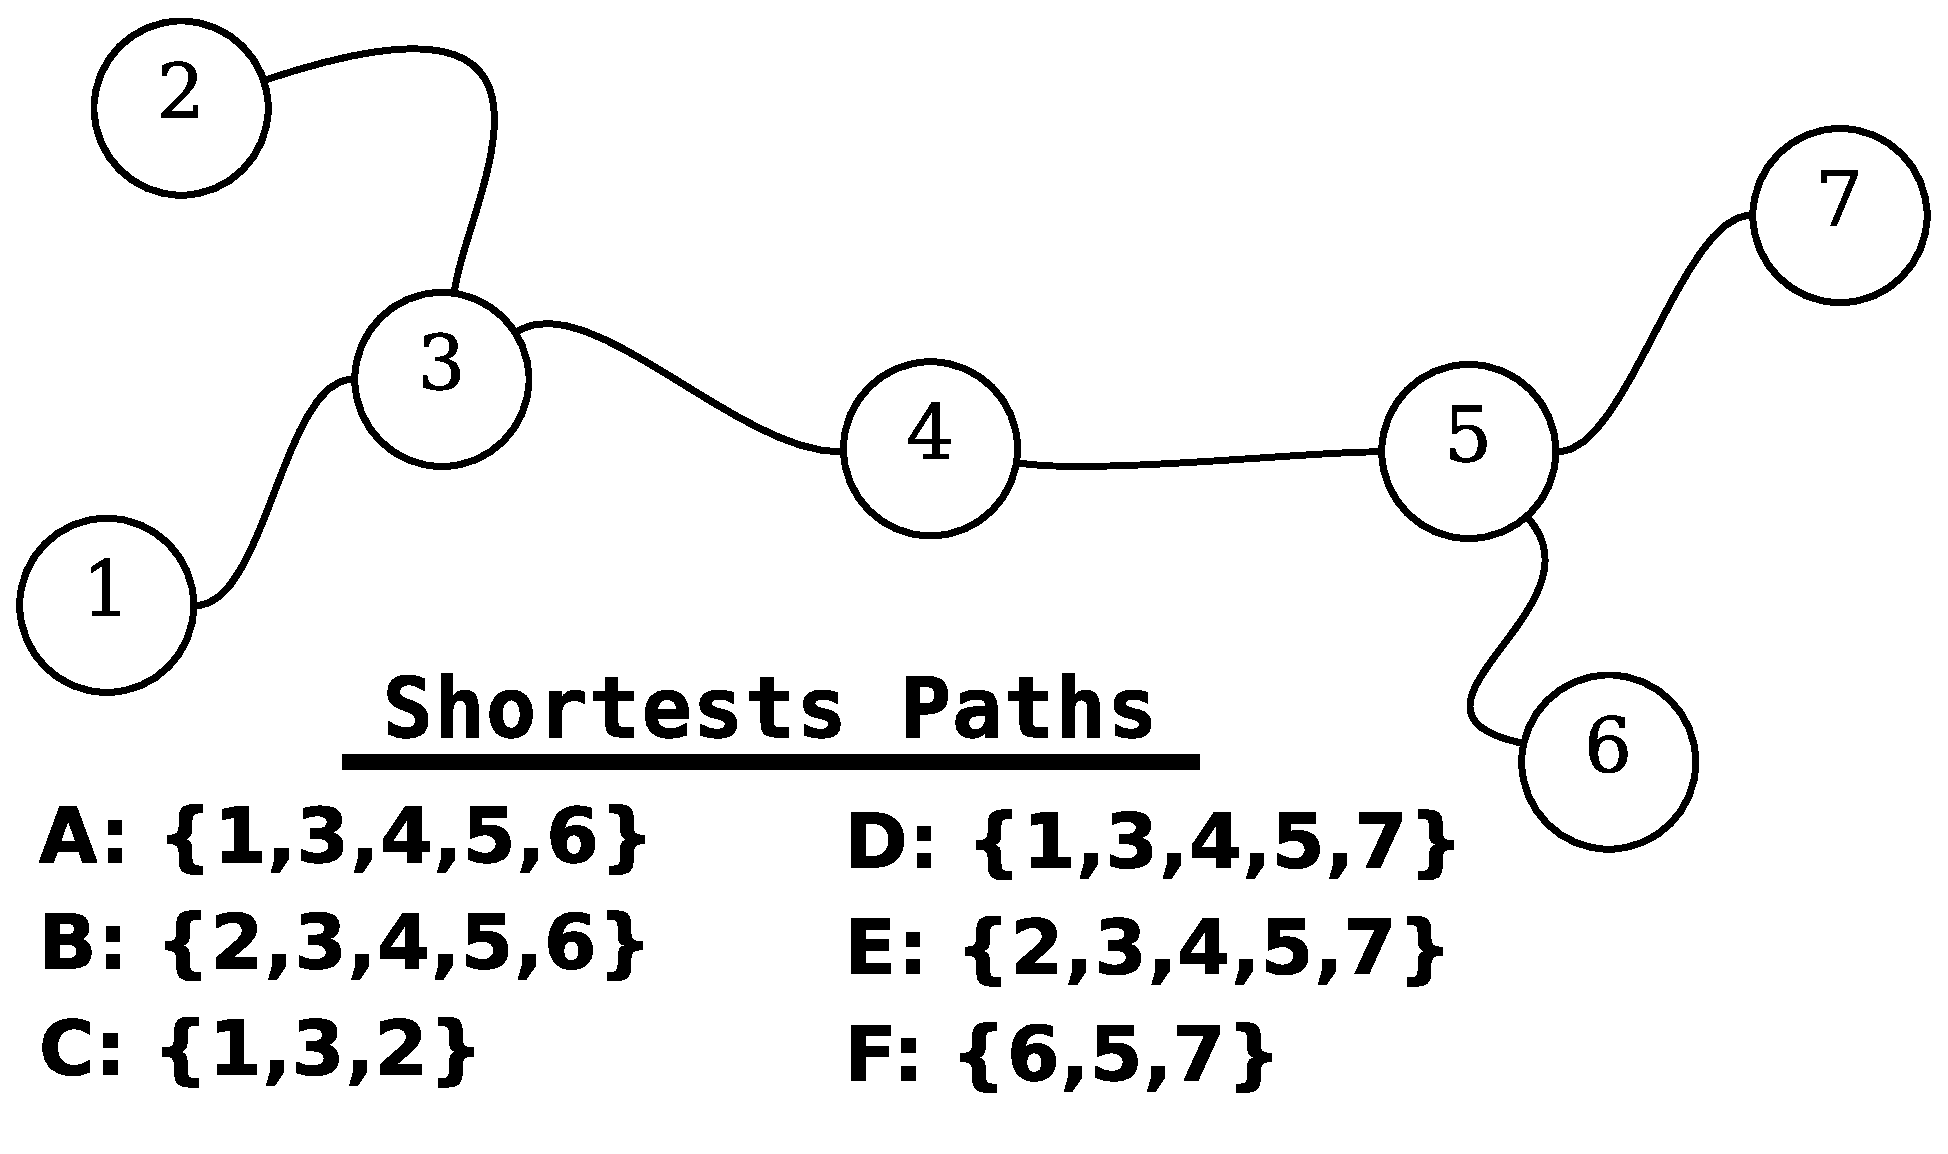
\includegraphics[width=0.5\textwidth]{figures/rxmap}
        \caption{Simple graph representation of a map.}
  \label{fig:rxmap}
\end{figure}


\subsection{Architecture}
We propose a system with a static \spath cache implemented in front of an existing \spath service (See fig. \ref{fig:routequery}) such that if the cache can answer a query then the result can be returned immediately. 

When the system receives a \spath query from a user (fig. \ref{fig:routequery}A) the system first checks if the cache (fig. \ref{fig:routequery}B) is able to answer the query. If the cache contains the query answer it is immediately returned (fig. \ref{fig:routequery}D), else the \spath algorithm is called (fig. \ref{fig:routequery}C) and the \spath result returned (fig. \ref{fig:routequery}D).

\begin{figure}
  \center
        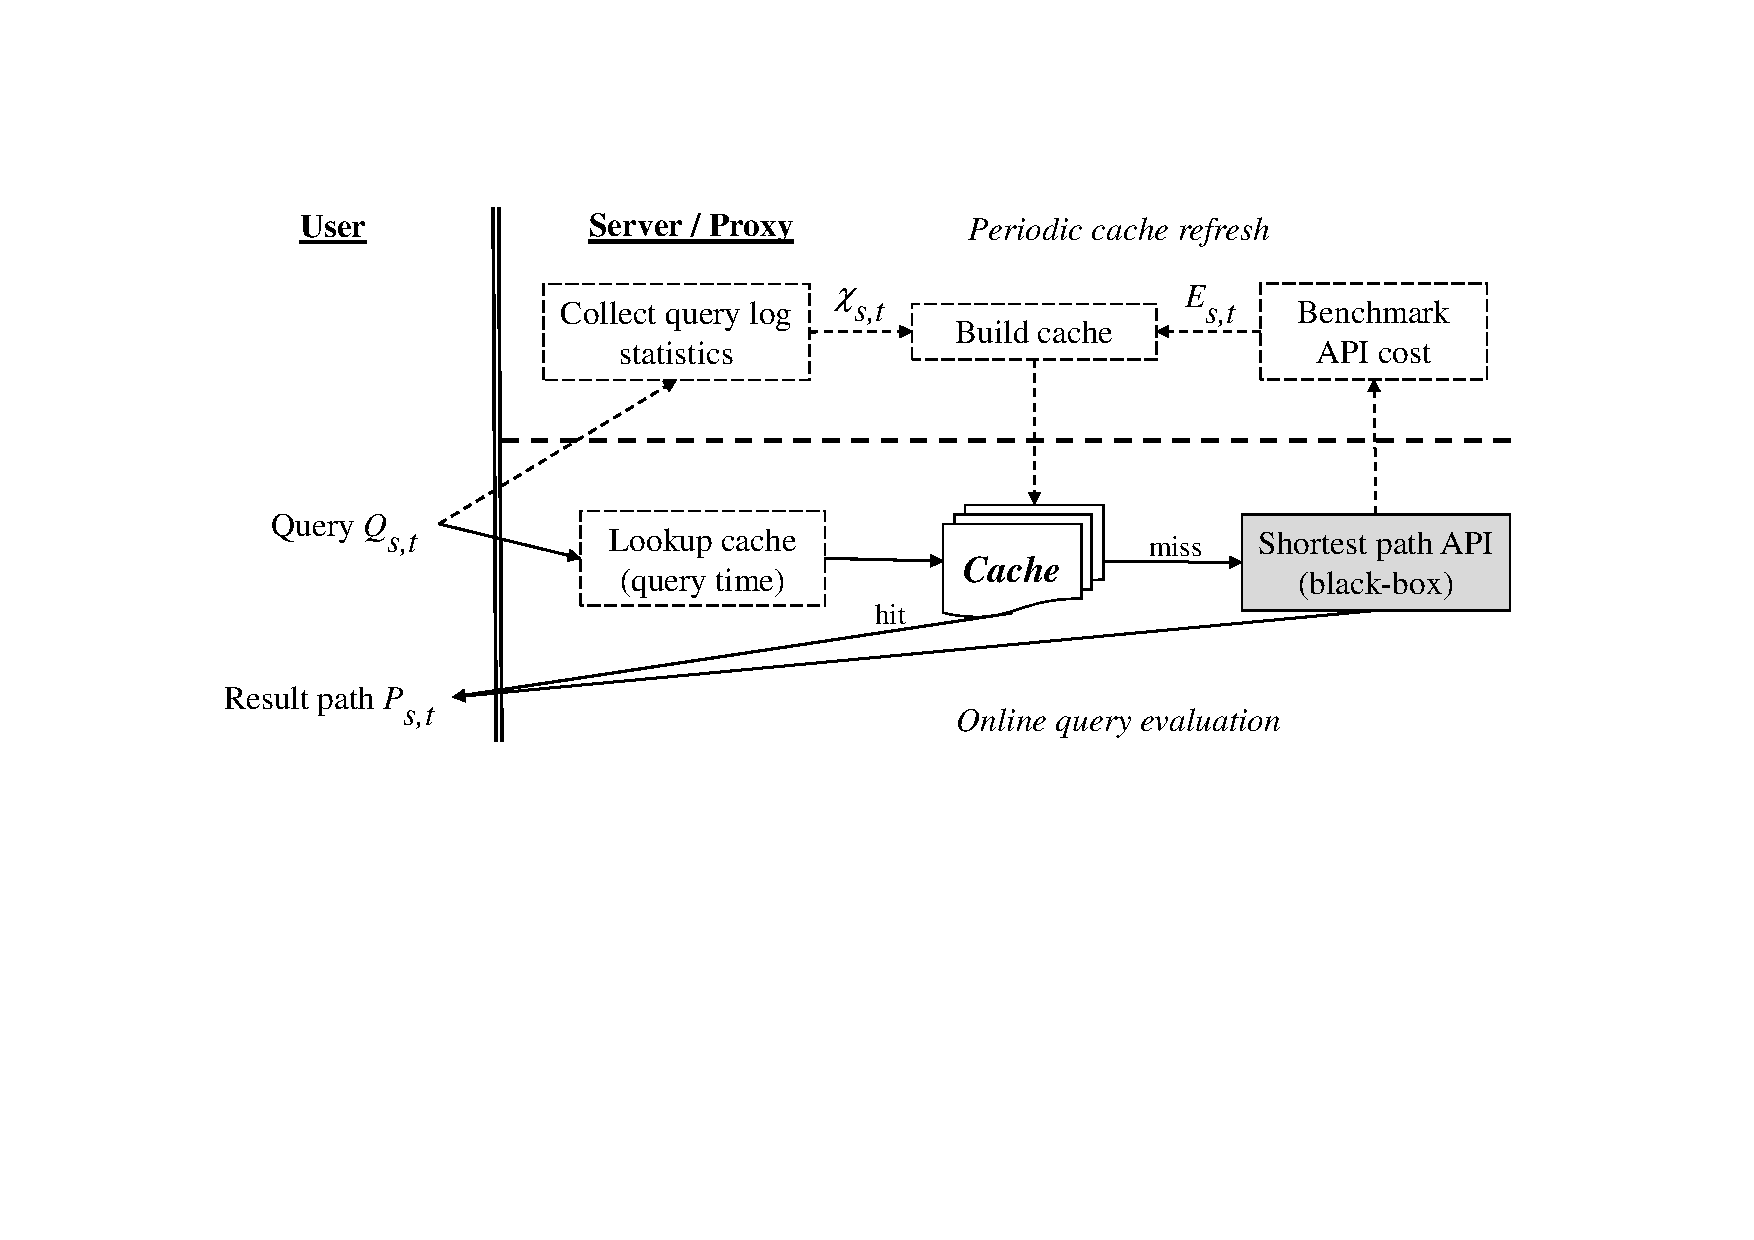
\includegraphics[width=0.5\textwidth]{figures/routequery}
        \caption{Buffer placement in \spath service providers system.}
  \label{fig:routequery}
\end{figure}


\subsection{Optimization Intend} \label{subsec:goals}

As the main problem with expensive \spath calculations is time needed, we use reduction in \textit{\cet} as the main optimization target and measurement to evaluate our success.
At a \spath service provider, the time spent to return a \spath result is essentially composed of two tasks: calculating the \spath and the overhead of query processing. 

We will address 3 subgoals:
\begin{enumerate}
\item \label{item:goal1}Reduce the gross \cet used to calculate \spathsns.
\item \label{item:goal2}Reduce the gross \cet spent on overhead in query processing.
\item \label{item:goal3}Determine the value of a sub-path in the cache.
\end{enumerate}

We want reduce the gross \cet of \spath calculations - goal 1 - as it is the most CPU intensive task at a \spath service, and therefor also the most time consuming. By using a cache we expect to see a negavite correlation between cache hit rate and \cet used on \spath calculation.

In a \spath service there will always be a some overhead associated with \spath query processing. Introducing a cache in front of the existing \spath service (fig. \ref{fig:routequery}B) will undeniably add more overhead as the cache needs to be queried for all queries submitted to the \spath service, regardless of whether it is able to answer the query or not. In order for the cache to be useful, the overhead introduced needs to be minimized (goal \ref{item:goal2}). We always have to make sure that the savings achieved by adding a cache to the system is greater than the overhead introduced.

The fact that the system will be using a static cache, and \spaths exhibit the \oss property, makes goal 3 - determining the value of a \spath subpath - very important. The ability to do goal \ref{item:goal3} well will have a direct influence on goal \ref{item:goal1} and  \ref{item:goal2}. If we fill the cache with useless \spaths we will end up calculating a \spath for all queries, as well as the overhead from checking the cache for each query. Solving goal 3 well is the most direct way to solve goal 1.

The \oss property states that every sub-path of a \spath is also a \spath. i.e \spath Q1 in table \ref{tab:queries} consists of: 
$\{Q_{1,3}, Q_{1,4}, Q_{1,5}, Q_{1,6}, Q_{3,4},$ $Q_{3,5}, Q_{3,6}, Q_{4,5}, Q_{4,6}, Q_{5,6}\}$, each one being a \spathns.

\begin{lemma}\label{lem:oss}
If a path $Q_{s,t}: v_s,v_{s+1},\ldots,v_t$ is a \spath, then $\forall$ $(v_k,v_l) | v_k \in Q_{s,t} \wedge v_l \in Q_{s,t}$ there is a  \spath $Q_{k,l}$ with start-/end-node in $v_k,v_l$, following a sub-path of $Q_{s,t}$ 
\end{lemma}

\begin{table}
\begin{tabular*}{\columnwidth}{|l||p{0.69\columnwidth}|}
\hline
\bf Abbreviation & \bf Meaning \\\hline
\spath          & Shortest Path \\\hline
$Q_{s,t}$	& \spathns: $\{v_s,v_{s+1},\ldots,v_t\}$ \\\hline
\acs{LRU}       & \acl{LRU} \\\hline
FIFO            & First In First Out \\\hline
\acs{SPS}       & \acl{SPS} \\\hline
\acs{CET}	& \acl{CET} \\\hline
\acs{OSS}	& \acl{OSS} \\\hline
\end{tabular*}
\caption{Table of Notation}
\label{tab:symbols}
\end{table}




% \subsection{helping text}
% \begin{enumerate}
% \item Introduce the problem setting in more detail than in the introduction and formally define the problem and what exactly we aim to solve in this paper.\\
% \item show where exactly the proposed cache is located in an online \spath service providers system.
% \item State goal 1(a) and 2(b)
% 	\begin{enumerate}
% 	\item Reduce the time spent executing the \spath algorithm. - The \spath algorithm is usually the single most CPU expensive task at a \spath service provider.
% 	\item Reduce the time spent on overhead. - Introducing a cache will also add some overhead, this overhead not desirable and should  be minimized.
% 	\end{enumerate}
% \item Introduce the overall setting which our solution work in and give a table of notation for reader reference.
% \end{enumerate}

\section{Introduction} % Bookmark information

\subsection{Overview} % Bookmark information, displayed in the progress tree

\begin{frame}[red] %hmm.. thought i could change colour here :S
\frametitle{Goals}

Goal one
\begin{itemize}
\item Remove user identifying information from trajectories.
\end{itemize}

\vspace{3em}
Goal two, following Goal one\\

\begin{itemize}
\item Ensure enough information after removal of user information that:
	\begin{itemize}
	\item Similar sub-trajectories used to get from point A to B can be found
	\item Analysis of which roads are congested, and when; can be performed.
	\end{itemize} 
\end{itemize}
\end{frame}

\subsection{Related work}

\begin{frame}
\frametitle{Related work}

  \begin{itemize}
\item Protection of Identifiers on Trajectories

\item Trajectory classification
\end{itemize}

\end{frame}


\begin{frame}[red] %hmm.. thought i could change colour here :S
\frametitle{Protection of Identifiers on Trajectories}
Post processing of trajectories
	\begin{itemize}	 
	\item  Add information
		\begin{itemize}
			\item Add fake trajectories
		\end{itemize}
	\item Remove information 
		\begin{itemize}
			\item Remove sensitive segments of trajectories 
			\item collapse similar trajectories into one
		\end{itemize}
	\end{itemize}
\end{frame}


% \begin{frame}[red] %hmm.. thought i could change colour here :S
% \frametitle{Trajectory classification}
% 
%   \begin{itemize}
% 	\item Similarity of trajectories
% 	\item Outlier detection
% 	\item Congestion analysis
%   \end{itemize}
% \end{frame}

%\subsection{Related Work} % Bookmark information, displayed in the progress tree


\begin{frame}[red] %hmm.. thought i could change colour here :S
\frametitle{Our vs. Existing Approaches }
FL\&VL versus existing privacy-aware proximity detection approaches:
\begin{center}  
	\begin{tabular}{| l | c | c | c |}
	\hline
	\textbf{Feature}		& \textbf{FL\&VL}	& \textbf{Solution 1}	& \textbf{Solution 2} \\ \hline 
	P2P comm.			&			&			& + \\ \hline
	Client-server comm		& +			&   +			& + \\ \hline
	Strength of privacy		& strong		& weak			& average \\ \hline		
	User settings flexibility	& high			& average		& average \\ \hline		
	\end{tabular}
\end{center}	

\end{frame}



% \begin{frame}[red] %hmm.. thought i could change colour here :S
% \frametitle{Anonymizers are not Necessary}
% Private Queries in Location Based Services: Anonymizers are not Necessary.
% \begin{itemize}
% \item Proposes a framework to support private location-dependent queries.
% \item Does not require an anonymizer, since it's a single point of attack.
% \item Uses cryptographic techniques to ensure privacy.
% \item Communication and CPU intense, because of encryption.
% \end{itemize}
% \end{frame}
% 
% 
% 
% \begin{frame}[red] %hmm.. thought i could change colour here :S
% \frametitle{Buddy Tracking}
% Buddy tracking - efficient proximity detection among mobile friends.
% \begin{itemize}
% \item Proposes a centralized server and a peer-to-peer method for tracking friends.
% \item Using the strips on the peer-to-peer algorithm - ensures privacy and reduces communication cost.
% \item Using a quadtree algorithm for the centralized algorithm.
% \item Still lot of communication using the peer-to-peer algorithm.
% \item Centralized server algorithm.has a lot of overhead and is outperformed when lots of users has joined the service.
% \item Privacy is not discussed in this article.
% \end{itemize}
%\end{frame}

 

%\subsection{FL vs. VL}

\begin{frame}[red] %hmm.. thought i could change colour here :S
\frametitle{FL vs. VL}
Differences between \textsc{FriendLocator} and \textsc{VicinityLocator}:
\begin{center}  
\begin{tabular}{| p{3cm} | p{3.5cm} | p{3.5cm} |}
\hline
\textbf{Feature}    & \textbf{\textsc{FriendLocator}}  & \textbf{\textsc{VicinityLocator}}   \\ 	  
  \hline
Notion of proximity & $dist(a,b)<\epsilon$   
\includegraphics[scale=0.4]{images/proxDet1.png}  & $loc(a) \in vic(b)$ \includegraphics[scale=0.2]{images/proxDet2.png} \\ 
\hline
User settings  & $\forall (a,b): \epsilon_{a,b}$ & $\forall a: vic(a)$, $\lambda(a)$,  \\
\hline
Quality of service (precision) & Depends on $\epsilon_{a,b}$	& $min(\lambda(a)$, $\lambda(b))$\\ 
  \hline	
Communication is traded for & $\epsilon$ and	precision & Precision   \\	
  \hline	
\end{tabular}
\end{center}	
\end{frame}


%\section{FriendLocator} % Bookmark information

\begin{frame}[red]
\frametitle{\textsc{FriendLocator}}
\begin{center}
\Large\textsc{FriendLocator} - A Location Privacy Aware Friend Locator
\end{center}
\end{frame}

\subsection{Core idea}
\begin{frame}[red]
\frametitle{Core idea of \textsc{FriendLocator}}
\only<1>{ 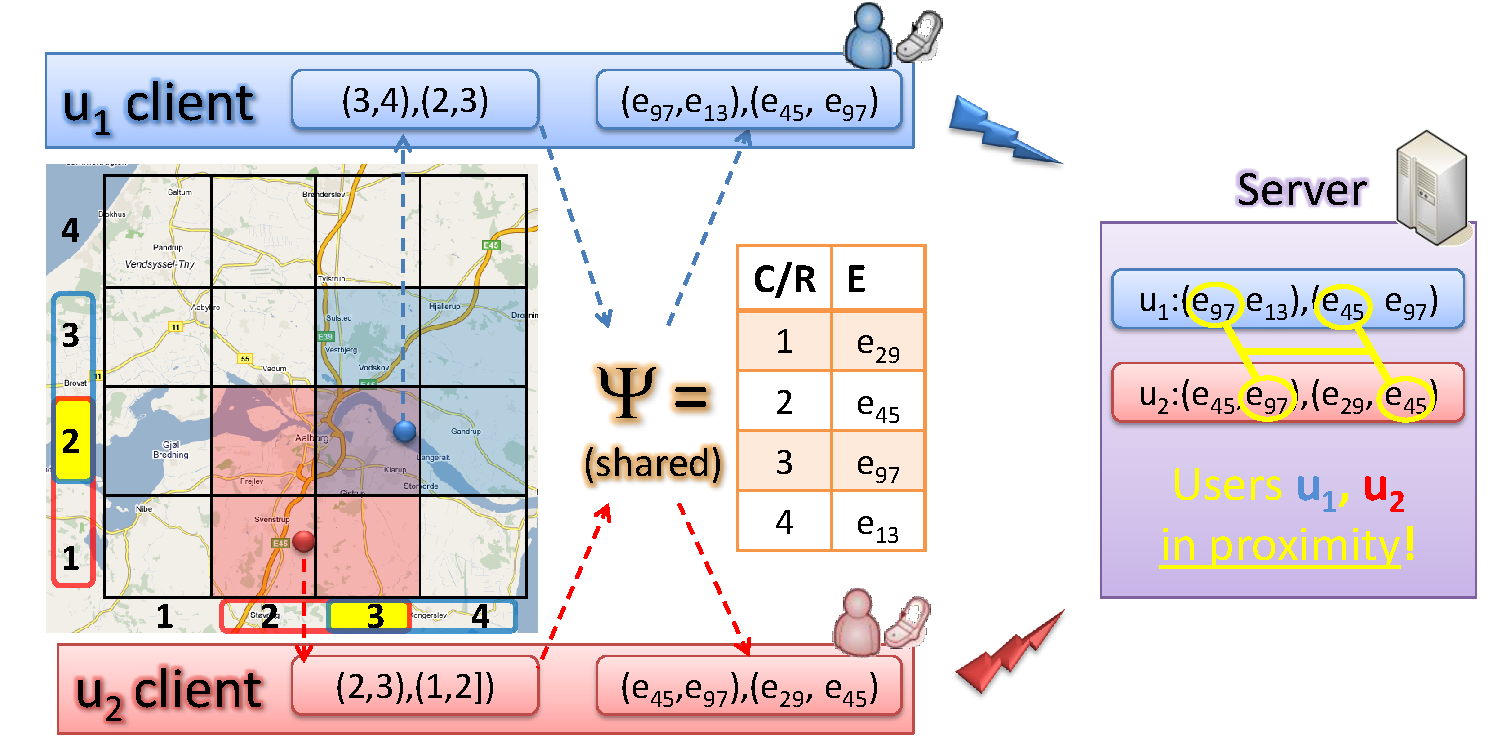
\includegraphics[scale=0.45]{images/ffBehaviour.pdf}}
\only<2>{ \includegraphics[page=7,scale=0.55]{images/imagesLRS.pdf}}
\only<3>{ \includegraphics[page=8,scale=0.55]{images/imagesLRS.pdf}}
\only<4>{ \includegraphics[page=9,scale=0.55]{images/imagesLRS.pdf}}
\only<5>{ \includegraphics[page=10,scale=0.55]{images/imagesLRS.pdf}}
\end{frame}

\begin{frame}[red]
\frametitle{Limitation and extensions of the idea}
Limitations of the core idea:
\begin{enumerate}
 \item Intercepted $\Psi$ opens location privacy leakage possibility
 \item A proximity detection distance is fixed ($2d\sqrt{2}$)  
\end{enumerate}
	\begin{tabular}{p{5cm} p{4cm}} 
	   \includegraphics[scale=0.2]{images/usrSrvAdversary.pdf} &
	   \includegraphics[scale=0.2]{images/usrPosDemoA.pdf} 
	\end{tabular}
	
Extensions, supported by \textsc{FriendLocator}:
\begin{enumerate}
   \item Grouping of friends
   \item Incremental Proximity Detection Approach
\end{enumerate}
\end{frame}

\subsection{Grouping of friends}

\begin{frame}[red]
\frametitle{Grouping of friends}
 Solution:
	\begin{itemize}
	\item Users are grouped into friend-groups			  
	\item A distinct $\Psi$ is assigned for every friend-group
	\end{itemize}
\begin{center}
  \includegraphics[page=11,scale=0.3]{images/imagesLRS.pdf}
\end{center}	
\vspace{-1cm}
Consequences:
	\begin{itemize}
	\item When user becomes malicious, users from common groups are endangered
	\end{itemize}
\end{frame}

\subsection{Incremental Proximity Detection Approach}
\begin{frame}[red]
\frametitle{Incremental Proximity Detection Approach}
\only<1>{
The solution:
	\begin{itemize}
	\item A list of grids with decreasing cell size is assigned for every friend-group
	\end{itemize}
\begin{center}
  \includegraphics[scale=0.2]{images/proxDet3.pdf} 
\end{center}	
Consequences:
	\begin{itemize}
	\item Any pair of friends in friend-group will be able to choose a preferred proximity distance
	\end{itemize}
}
\only<2>{\includegraphics[page=13,scale=0.55]{images/imagesLRS.pdf}}
\only<3>{\includegraphics[page=14,scale=0.55]{images/imagesLRS.pdf}}
\only<4>{\includegraphics[page=15,scale=0.55]{images/imagesLRS.pdf}}
\only<5>{\includegraphics[page=16,scale=0.55]{images/imagesLRS.pdf}}
\only<6>{\includegraphics[page=17,scale=0.55]{images/imagesLRS.pdf}}
\only<7>{\includegraphics[page=18,scale=0.55]{images/imagesLRS.pdf}}
\only<8>{\includegraphics[page=19,scale=0.55]{images/imagesLRS.pdf}}
\end{frame}

%\section{Problem}\label{sec:problem}

In our setting we assume users own an Internet enabled mobile device with positioning capabilities. Users issue \spath queries to an online service provider. Users want the response time, on the return of their \spath result, to be comparable to that of an offline application. We use the terms user query, incoming query, and query interchangeably.

The \spath service provider needs to provide a fast service to its users. The service provider also want to save cost on hardware, such as CPU and HDD space. The \spath provider therefor wants to return as many \spath results as possible, using the least amount of computation and space.

Calculating a \spath will, regardless of the algorithm used, always be an expensive calculation\cite{CNeed}. Using a \spath cache at the \spath service provider can reduce the CPU cycles used in order to return a \spath result. Doing so would at the same time also increase the response time of the \spath service, as saving CPU cycles not only allows for more \spaths to be computed on the same hardware, but also allows for returning a cached result much faster than it would be possible if the \spath had to be calculated first.

A \spath has the property of \oss (see lemma \ref{lem:oss}) which means that any \spath in the cache can answer any \spath query where both origin and target node are on the \spathns. Calculating which \spathsns, and their sub-paths, provide the most benefit will obviously be necessary for optimal utilization of the cache. A static cache, which is populated in an offline phase (fig. \ref{fig:routequery}E), is used. A static cache will impose minimal overhead to query processing. Section \ref{sec:competitors} explains why we choose a static cache.

The properties of \ossns (Lemma \ref{lem:oss}) states that all sub-paths on a \spath are also \spathsns. Using \spath Q1 in table \ref{tab:queries} we would also be able to a query from $v_3$ to $v_5$, or $v_4$ to $v_6$ (See fig. \ref{fig:rxmap}), as these nodes are part of Q1. The same of cause also holds for any \spath Q1-Q6 from table \ref{tab:queries}.

\begin{figure}[hbt]
  \center
        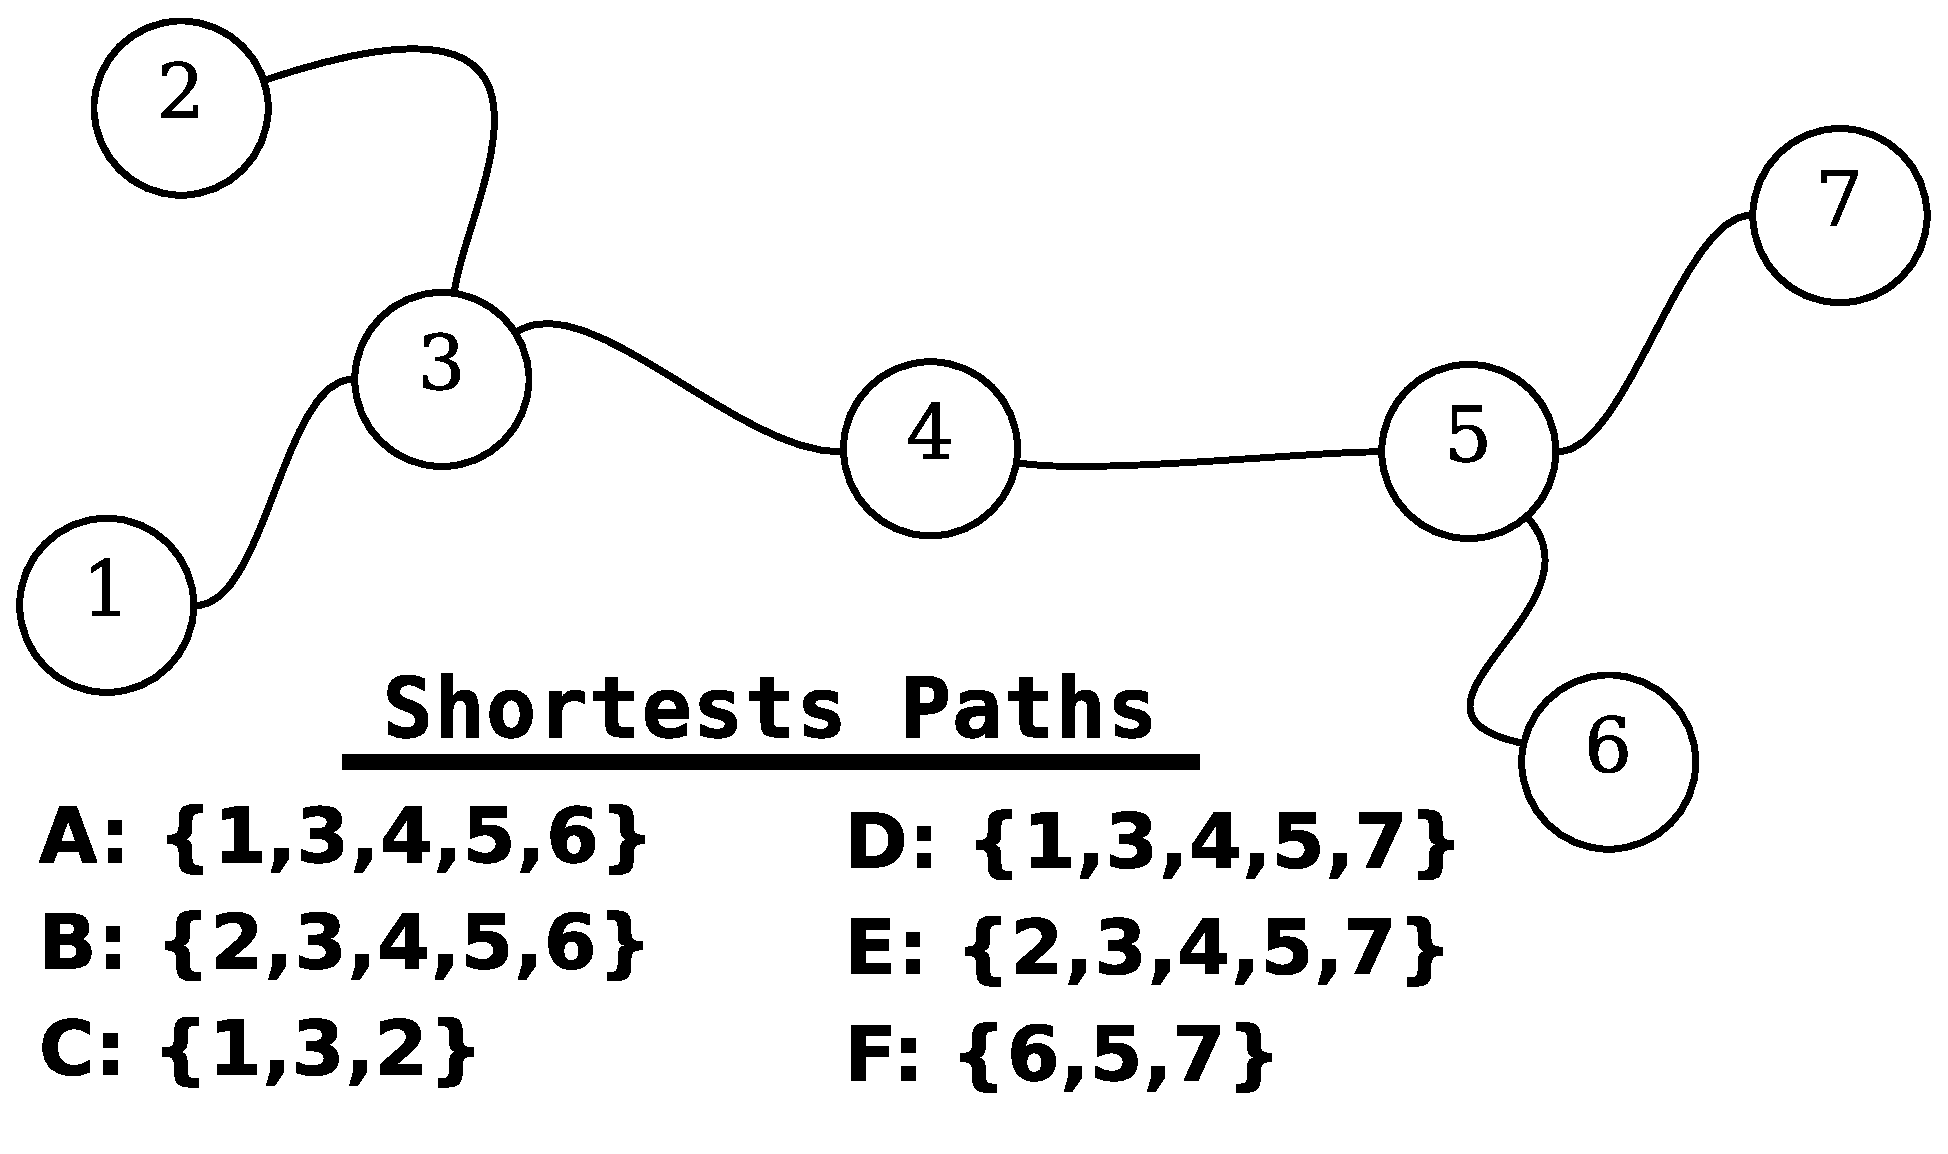
\includegraphics[width=0.5\textwidth]{figures/rxmap}
        \caption{Simple graph representation of a map.}
  \label{fig:rxmap}
\end{figure}


\subsection{Architecture}
We propose a system with a static \spath cache implemented in front of an existing \spath service (See fig. \ref{fig:routequery}) such that if the cache can answer a query then the result can be returned immediately. 

When the system receives a \spath query from a user (fig. \ref{fig:routequery}A) the system first checks if the cache (fig. \ref{fig:routequery}B) is able to answer the query. If the cache contains the query answer it is immediately returned (fig. \ref{fig:routequery}D), else the \spath algorithm is called (fig. \ref{fig:routequery}C) and the \spath result returned (fig. \ref{fig:routequery}D).

\begin{figure}
  \center
        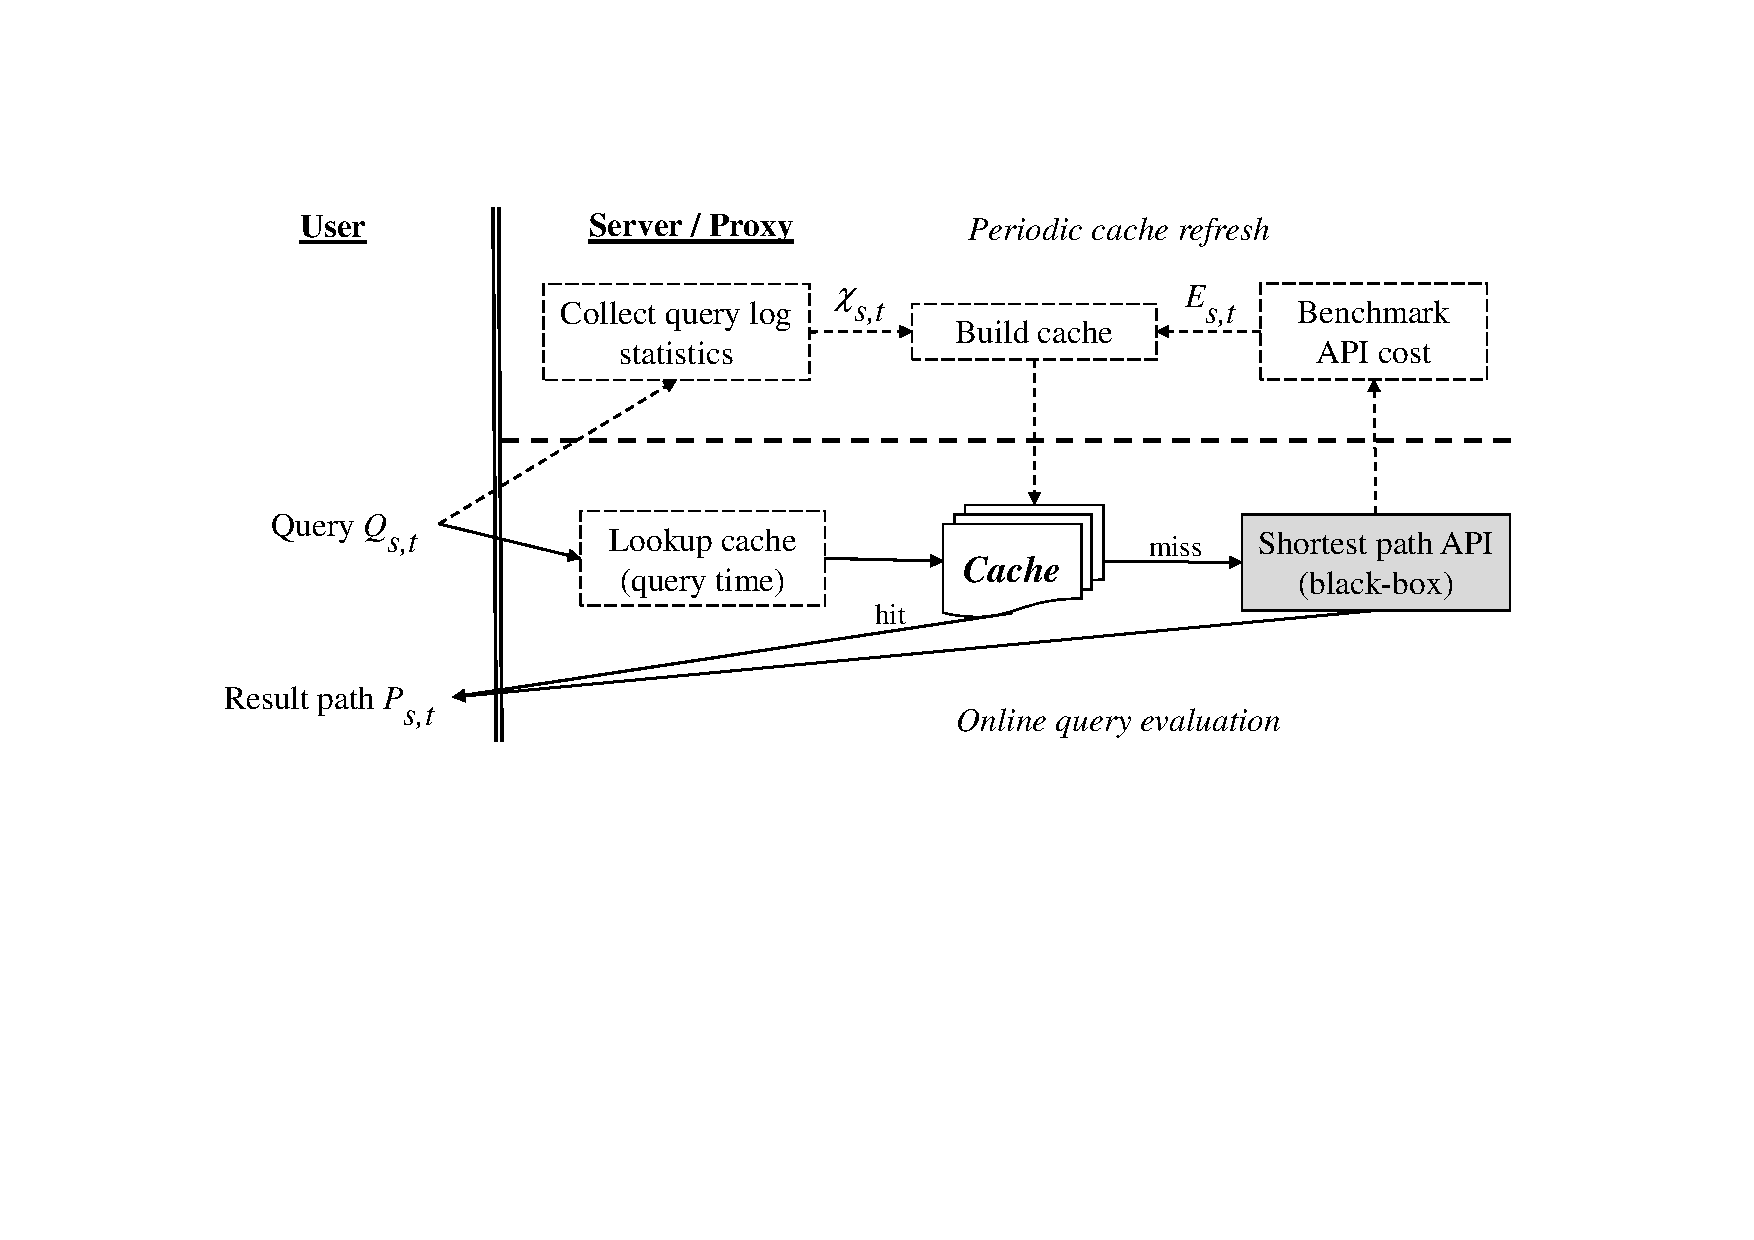
\includegraphics[width=0.5\textwidth]{figures/routequery}
        \caption{Buffer placement in \spath service providers system.}
  \label{fig:routequery}
\end{figure}


\subsection{Optimization Intend} \label{subsec:goals}

As the main problem with expensive \spath calculations is time needed, we use reduction in \textit{\cet} as the main optimization target and measurement to evaluate our success.
At a \spath service provider, the time spent to return a \spath result is essentially composed of two tasks: calculating the \spath and the overhead of query processing. 

We will address 3 subgoals:
\begin{enumerate}
\item \label{item:goal1}Reduce the gross \cet used to calculate \spathsns.
\item \label{item:goal2}Reduce the gross \cet spent on overhead in query processing.
\item \label{item:goal3}Determine the value of a sub-path in the cache.
\end{enumerate}

We want reduce the gross \cet of \spath calculations - goal 1 - as it is the most CPU intensive task at a \spath service, and therefor also the most time consuming. By using a cache we expect to see a negavite correlation between cache hit rate and \cet used on \spath calculation.

In a \spath service there will always be a some overhead associated with \spath query processing. Introducing a cache in front of the existing \spath service (fig. \ref{fig:routequery}B) will undeniably add more overhead as the cache needs to be queried for all queries submitted to the \spath service, regardless of whether it is able to answer the query or not. In order for the cache to be useful, the overhead introduced needs to be minimized (goal \ref{item:goal2}). We always have to make sure that the savings achieved by adding a cache to the system is greater than the overhead introduced.

The fact that the system will be using a static cache, and \spaths exhibit the \oss property, makes goal 3 - determining the value of a \spath subpath - very important. The ability to do goal \ref{item:goal3} well will have a direct influence on goal \ref{item:goal1} and  \ref{item:goal2}. If we fill the cache with useless \spaths we will end up calculating a \spath for all queries, as well as the overhead from checking the cache for each query. Solving goal 3 well is the most direct way to solve goal 1.

The \oss property states that every sub-path of a \spath is also a \spath. i.e \spath Q1 in table \ref{tab:queries} consists of: 
$\{Q_{1,3}, Q_{1,4}, Q_{1,5}, Q_{1,6}, Q_{3,4},$ $Q_{3,5}, Q_{3,6}, Q_{4,5}, Q_{4,6}, Q_{5,6}\}$, each one being a \spathns.

\begin{lemma}\label{lem:oss}
If a path $Q_{s,t}: v_s,v_{s+1},\ldots,v_t$ is a \spath, then $\forall$ $(v_k,v_l) | v_k \in Q_{s,t} \wedge v_l \in Q_{s,t}$ there is a  \spath $Q_{k,l}$ with start-/end-node in $v_k,v_l$, following a sub-path of $Q_{s,t}$ 
\end{lemma}

\begin{table}
\begin{tabular*}{\columnwidth}{|l||p{0.69\columnwidth}|}
\hline
\bf Abbreviation & \bf Meaning \\\hline
\spath          & Shortest Path \\\hline
$Q_{s,t}$	& \spathns: $\{v_s,v_{s+1},\ldots,v_t\}$ \\\hline
\acs{LRU}       & \acl{LRU} \\\hline
FIFO            & First In First Out \\\hline
\acs{SPS}       & \acl{SPS} \\\hline
\acs{CET}	& \acl{CET} \\\hline
\acs{OSS}	& \acl{OSS} \\\hline
\end{tabular*}
\caption{Table of Notation}
\label{tab:symbols}
\end{table}




% \subsection{helping text}
% \begin{enumerate}
% \item Introduce the problem setting in more detail than in the introduction and formally define the problem and what exactly we aim to solve in this paper.\\
% \item show where exactly the proposed cache is located in an online \spath service providers system.
% \item State goal 1(a) and 2(b)
% 	\begin{enumerate}
% 	\item Reduce the time spent executing the \spath algorithm. - The \spath algorithm is usually the single most CPU expensive task at a \spath service provider.
% 	\item Reduce the time spent on overhead. - Introducing a cache will also add some overhead, this overhead not desirable and should  be minimized.
% 	\end{enumerate}
% \item Introduce the overall setting which our solution work in and give a table of notation for reader reference.
% \end{enumerate}

\section{Privacy Profile}

\begin{frame}[red]
\frametitle{Privacy Profile}
\begin{itemize}
\item Settings
\item t-anonymity
\item PSR
\item Protection types and schemes
\end{itemize}
\end{frame}

\subsection{Settings} % Bookmark information, displayed in the progress tree

\begin{frame}[red] %hmm.. thought i could change colour here :S
\frametitle{Settings}

Users Can
\begin{itemize}
	\item Set both globally and locally
	\begin{itemize}
		\item Temporal sensitivity
		\item Spatial sensitivity
	\end{itemize}
	\item Define a PSR
	\item Have multiple profiles.
\end{itemize}

\vspace{1em}
\begin{definition}[Privacy Profile]
$\left(stime,etime,d_s, d_t,\{PSR \} \right)$
\end{definition}

\end{frame}



\subsection{PSR} % Bookmark information, displayed in the progress tree


\begin{frame}[red] %hmm.. thought i could change colour here :S
\frametitle{PSR}

\begin{definition}[PSR]
A PSR $p$ is a tuple $(p_{edges}, d_s, d_t, class)$ where $p_{edges}$ is the set of tuples $\{(e, e_{from}, e_{to} | 0 \leq e_{from} < e_{to} \leq e_{length})\}$ which is sensitive. 
$e \in \mathbf{E}$ and $e_{from}, e_{to}, e_{length} \in \mathbb{R}$. 
$e_{from}/e_{to}$ specifies on $e$ the start-/end-location covered by $p_{cover}$. If $e$ is fully included in $p_{cover}$, $e_{from}/e_{to}$ is equal to $0/p_{length}$.
$d_s, d_t, class \in \mathbb{N}$ is respectively the spatial sensitivity, the temporal sensitivity, and the PSR classification
\end{definition}

\end{frame}

\begin{frame}[red] %hmm.. thought i could change colour here :S
\frametitle{PSR Classes}

\begin{table}
%\begin{tabular*}{0.8\columnwidth}{|p{0.2\columnwidth}|l|p{0.25\columnwidth}|}
\begin{tabular}{|l|l|}
\hline
\bf Classification	& \bf Scheme \\\hline		
Public Service Point	& AS \\\hline
House			& ASTI,RS \\\hline
Route w. endpoints	& AS, ASTI, RS  \\\hline
Route w/o endpoints	& AS, ASTI, RS  \\\hline
\end{tabular}
\end{table}
\vspace{1em}

Protection Schemes
\begin{itemize}
	\item AS - Always Sensitive.
	\item ASTI - Always Sensitive within a time interval.
	\item RS - Rarely Sensitive.
\end{itemize}
\end{frame}


\subsection{Time Period}
\begin{frame}[red]
\frametitle{Time Period}
\begin{columns}
	\begin{column}{0.5\textwidth}
		\only<1>{ 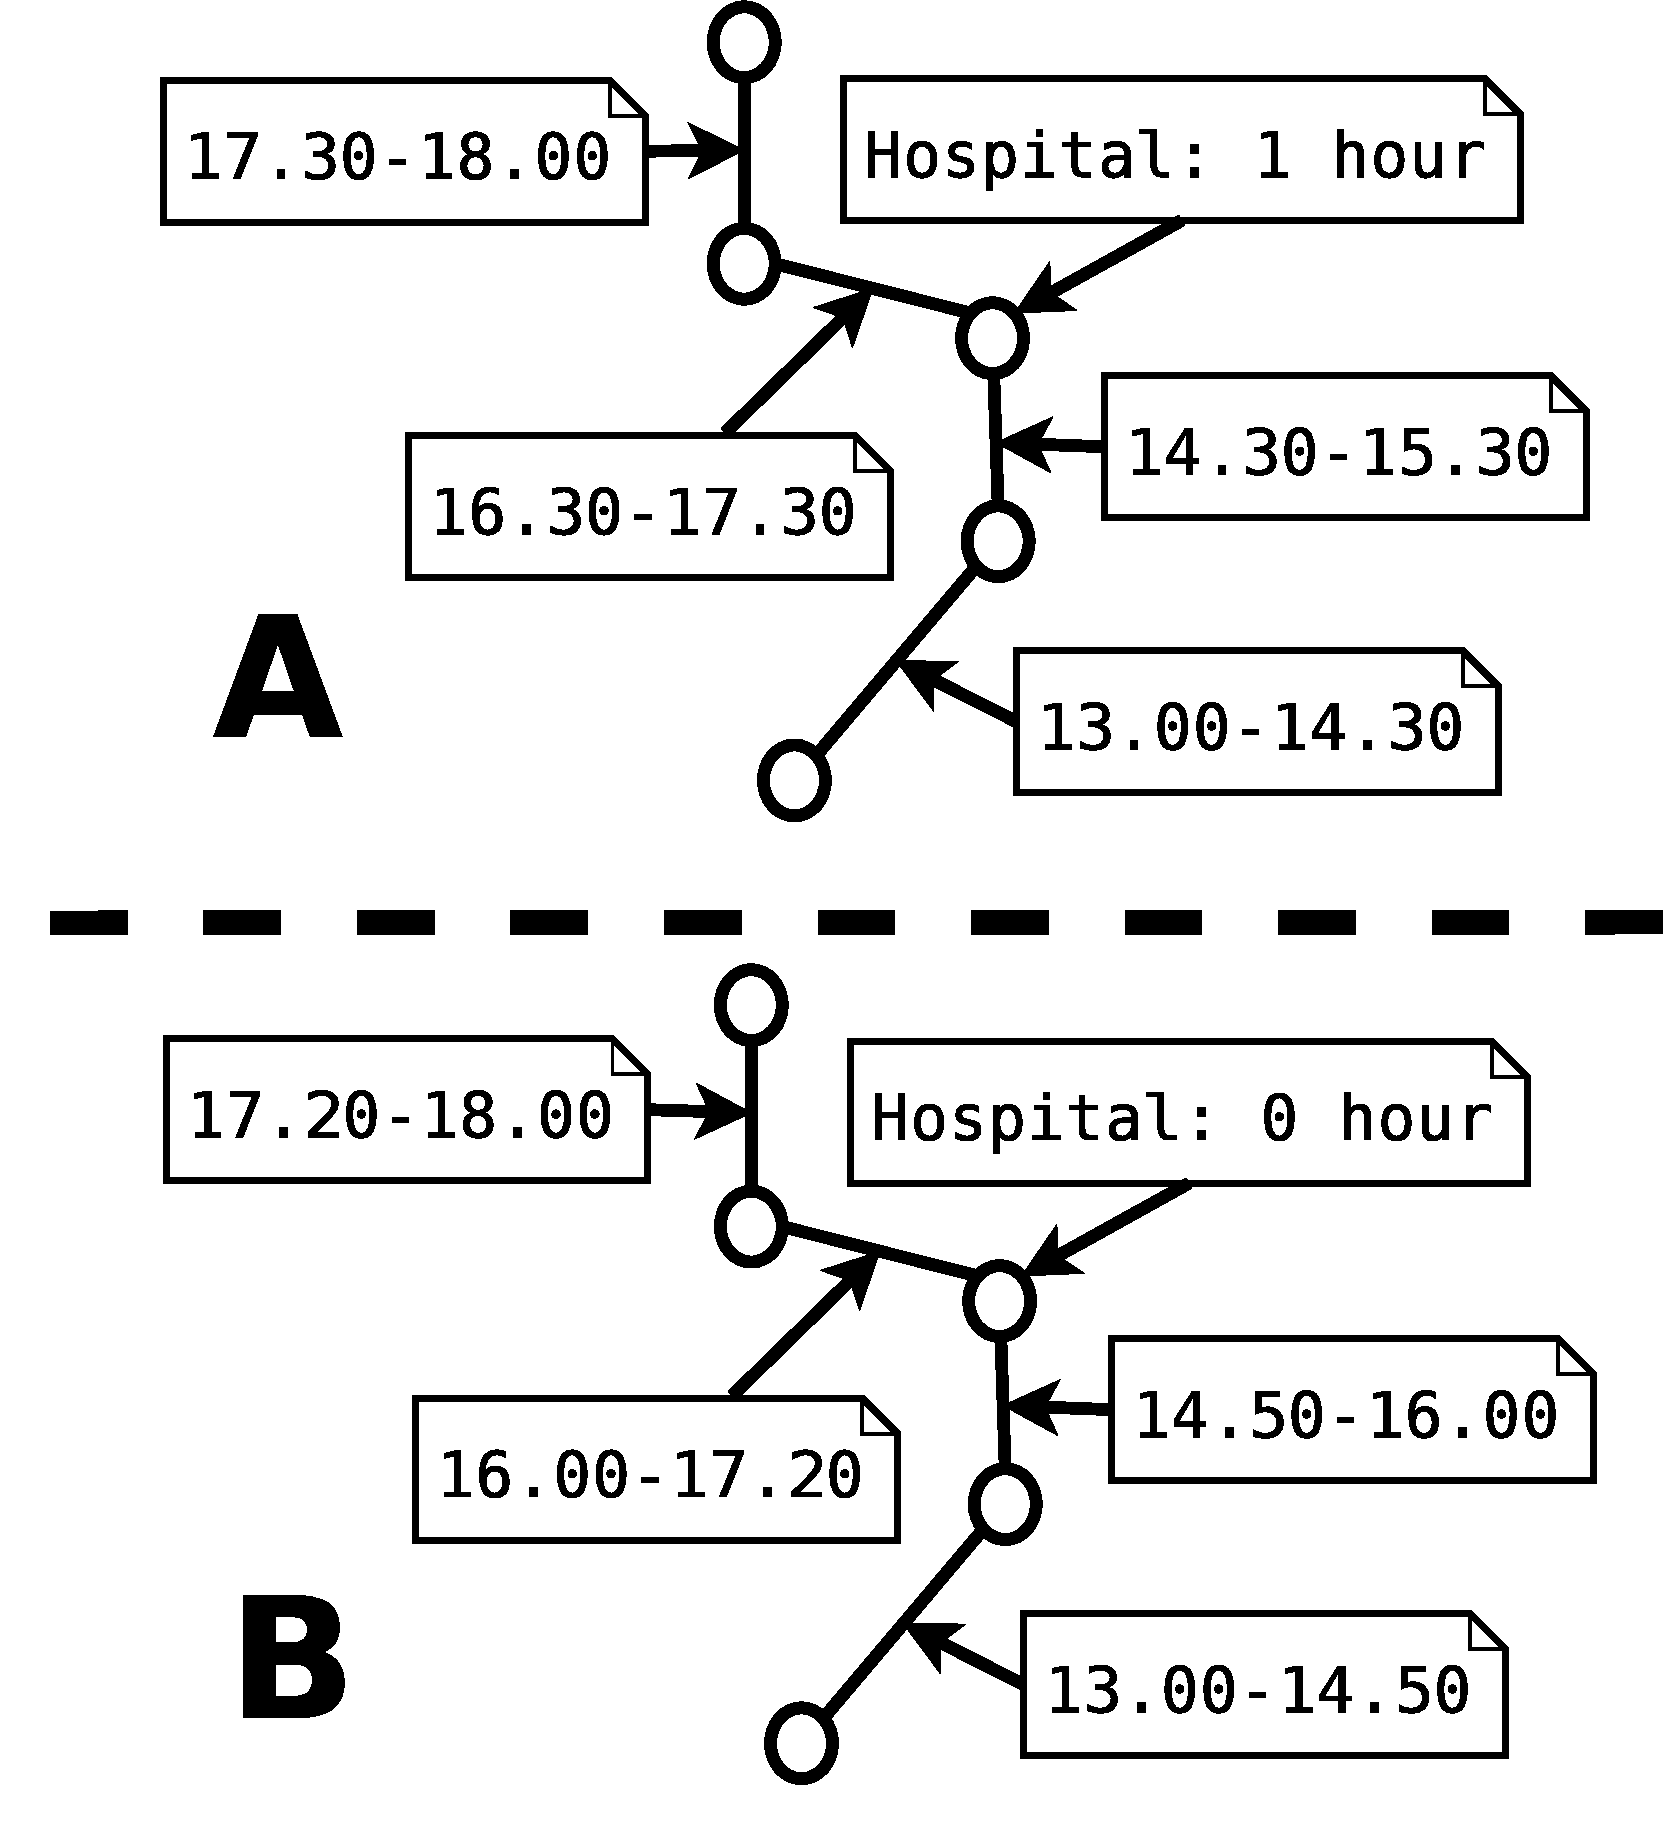
\includegraphics[scale=0.16]{images/trajecAdjustTime.pdf}}
	\end{column}
	\begin{column}{0.5\textwidth}
		\only<1>{ 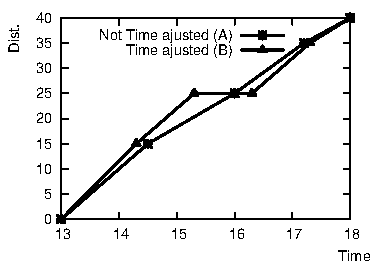
\includegraphics[scale=0.8]{images/trajecAdjustTimeGraph.pdf}}
	\end{column}
\end{columns}

\end{frame}

\subsection{t-anonymity} 
\begin{frame}[red] %hmm.. thought i could change colour here :S
\frametitle{t-anonymity}
\begin{definition}[t-anonymity]
Given $\mathbf{T}$, the set of trajectories and $p_{edges}$, the set of edges covering a sensitive part of trajectory $\gamma$. 

Let $\Gamma \subseteq \mathbf{T}$ be all trajectories which subtrajectories intersect with $p_{edges}$. $\Gamma' \subseteq \Gamma$ be all trajectories where, for edges intersecting with $p_{edges}$, at each timestamp of $\gamma$ their timestamps lie within a time period $TP$ symmetric around the timestamp of $\gamma$.

$\Gamma'$ is said to satisfy t-anonymity with respect to $TP$ and $\gamma$ iff $\Gamma'$ contains at least $t-1$ other trajectories.
\end{definition}
\end{frame}
\section{Algorithms}

\begin{frame}
\frametitle{Algorithm}

\begin{algorithm}[H]
\dontprintsemicolon
\SetVline

\SetKwInOut{Input}{input}\SetKwInOut{Output}{output}\SetKw{Return}{return}

% \Input
% {
% 
% 	$\mathbf{T}$: The set of trajectories $t$ \;
% 	$\mathbf{S}$: The set of privacy profiles $s$\;
% 	$G(\mathbf{V,E})$: Roadnetwork Graph \;
% 	$D \in \mathbb{R}$: Tolerance for how much a modified trajectory is allowed to diveate from original trajectory. \;
% 	$n \in \mathbb{N}$: Factor on how finegrained the road difference calculations should be \;
% 	{PS:} the set of all PSR \;
% }

%$\alpha \leftarrow t | t \in \mathbf{T} \wedge psr.p_{edges} \cap t \neq \emptyset $
\While{$ $Sensitive unanonymized edges exist}
{
	$\alpha \leftarrow {\bf Choose\_\alpha(\mathbf{T}, PS)}$ \;
	$PSRcand \leftarrow {\bf FindCand(\alpha, PS)}$ \;
	$calcCand~\leftarrow~{\bf CalcCand}(PSRcand, \alpha, D, n)$ \;
	$sortCand \leftarrow$  Sort $calcCand$ using ordering given by {\bf CompareCand()} \;
	$anonData \leftarrow anonData \cup {\bf AnonCand}(sortCand, \alpha$) \;
}
\(anonData \cup \{\forall t_i  \in t  | t \in \mathbf{T}\}, t_i \) is a subtrajectory that has not been modified or otherwise included during anonymization.

% \funcc{Choose$\_\alpha$}{\mathbf{T}, PS}
% {
% 	Choose a 4-tuple $\alpha: (t, t_{se}, d_{t}, d_{s})$. $\alpha.t$ is at least partially covered by the PSR $psr \in PS$. $PS$ is ordered by protection schemes from top to bottom. Within a protection scheme grouping $PS$ is sorted by the highest sensitivity, using ordering from {\bf CompareCand()}. If more than one candidate for $\alpha$ is found the first found will be chosen. \; 
% 
% 	\Return{$\alpha$}
% }


\end{algorithm}
\end{frame}

\begin{frame}
\frametitle{TrajecoriesPSR}

\begin{algorithm}[H]
{\bf TrajectoriesPSR}({$P, \mathbf{T}, \alpha$})

	$u \leftarrow$ {\bf PSRtoUser}(P) \tcp{\emph{user $(id,s,\{t\})$ where $P \in s.\{PSR\}$}}
 
 	$tSet \leftarrow \{(t, t_{se}, d_t, d_s) | \forall t \in \mathbf{T} \wedge t \cap \alpha.t \neq \emptyset \wedge P.p_{edges} \cup t \neq \emptyset \wedge t_{se} = \alpha.t \cap t \wedge t \in u.t, d_t = P.d_t, d_s = P.d_s \wedge \forall i,j | \alpha.t_{se}[i]_{\tau_{s}}-\frac{\alpha.d_t}{2} \leq t_{se}[j]_{\tau_{s}} \leq \alpha.t_{se}[i]_{\tau_{s}}+\frac{\alpha.d_t}{2} \}$

 	%$t \in \mathbf{T}$. At least one edge in $t$ is covered by P.$p_{edges}$ and $t \bigcap \alpha \neq \emptyset$. The returned tuple include $d_t,d_s,$ and $t_{se} = \alpha \bigcap t$.
 	\Return {$tSet$}

\end{algorithm}
\end{frame}
%% \subsection{Dynamic Solution} % Bookmark information, displayed in the progress tree
% \begin{frame}[red] %hmm.. thought i could change colour here :S
% \frametitle{Ze Introduction}
% 
% \begin{theorem}
%   In a right triangle, the square of hypotenuse equals
%   the sum of squares of two other sides.
% \end{theorem}
% 
%   Things in a Bulleted List\pause
%   \begin{itemize}
%   \item Bullets that\pause
%   \item Come up\pause
%   \item One by one %leave out the \pause on the final item
%   \end{itemize}
%   
% \end{frame}
%\section{User Profile}

\subsection{Proximity Approach}

\begin{frame}[red] %hmm.. thought i could change colour here :S
\frametitle{Motivation}
\textsc{FriendLocator}
\begin{itemize}
	\item the Proximity Detection Guaranties is to weak $(2d\sqrt{2})$
	\item is too inflexible - privacy \& precision not independent.
\end{itemize}

\vspace{2em}

Want solution independent of how the space it partitioned
\end{frame}

\subsection{Improvements}

\begin{frame}[red] %hmm.. thought i could change colour here :S
\frametitle{Improvements}

New features and improvements in \textsc{VicinityLocator}
\begin{columns}
\begin{column}{0.5\textwidth}
\begin{itemize}
	\item Granules (and rasterasation) 
	\item Better guaranties
	\item Ajustable vicinity
\end{itemize}
\vspace{5cm}
\end{column}
\begin{column}{0.5\textwidth}
\pgfputat{\pgfxy(0,0)}{\pgfbox[left,top]{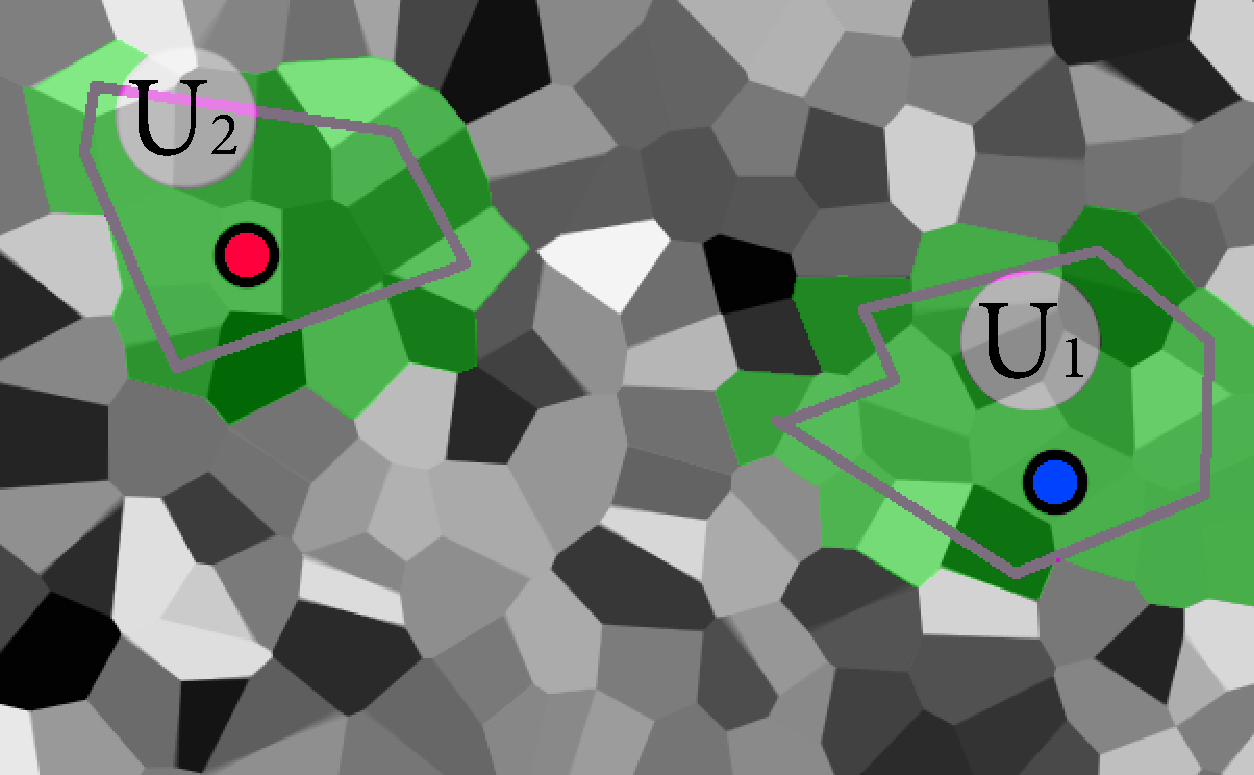
\includegraphics[width=\textwidth]{images/granVic}}}
\end{column}
\end{columns}
\end{frame}



% \subsection{VicinityLocator Examples}
% \begin{frame}[red] %hmm.. thought i could change colour here :S
% \frametitle{Demo of \textsc{VicinityLocator}}%r=500
% 	\only<1>{ 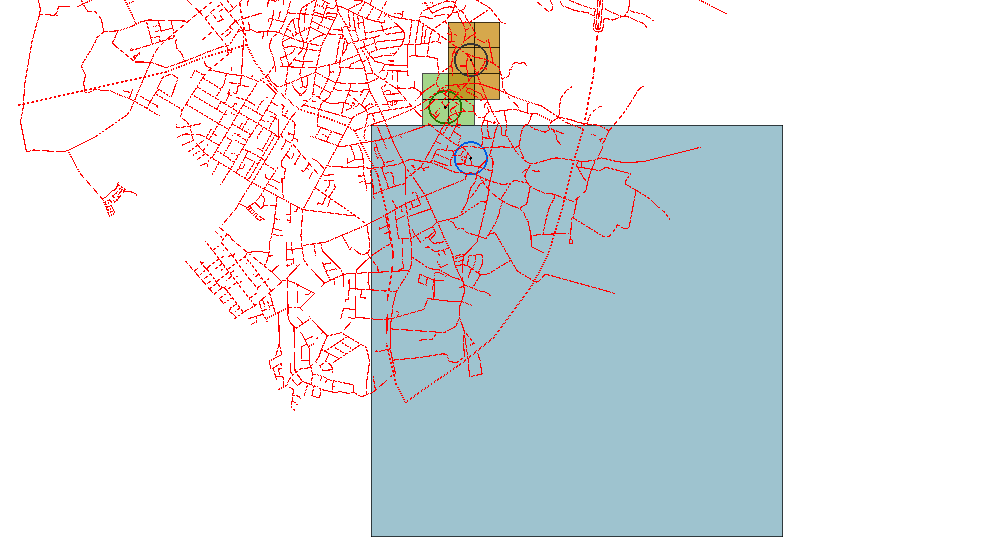
\includegraphics[page=1,scale=0.70]{images/demoVL/dump1.pdf}}
% 	\only<2>{ 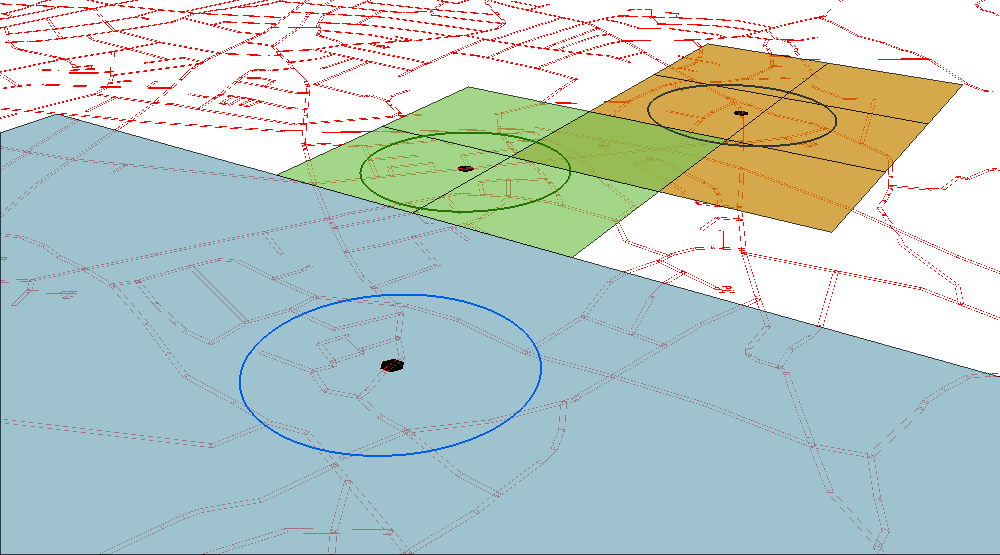
\includegraphics[page=1,scale=0.70]{images/demoVL/dump2.pdf}}
% 	\only<3>{ 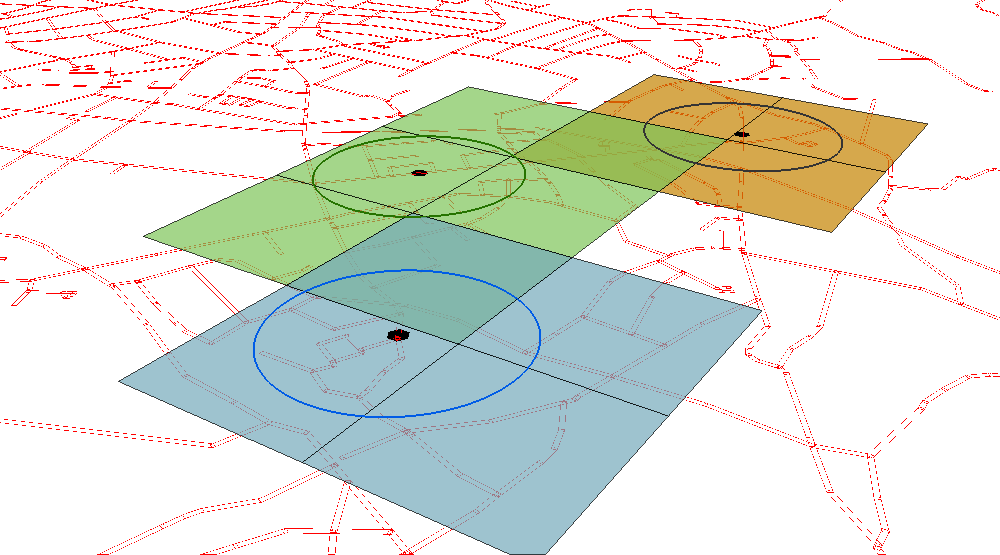
\includegraphics[page=1,scale=0.70]{images/demoVL/dump3.pdf}}
% 	\only<4>{ 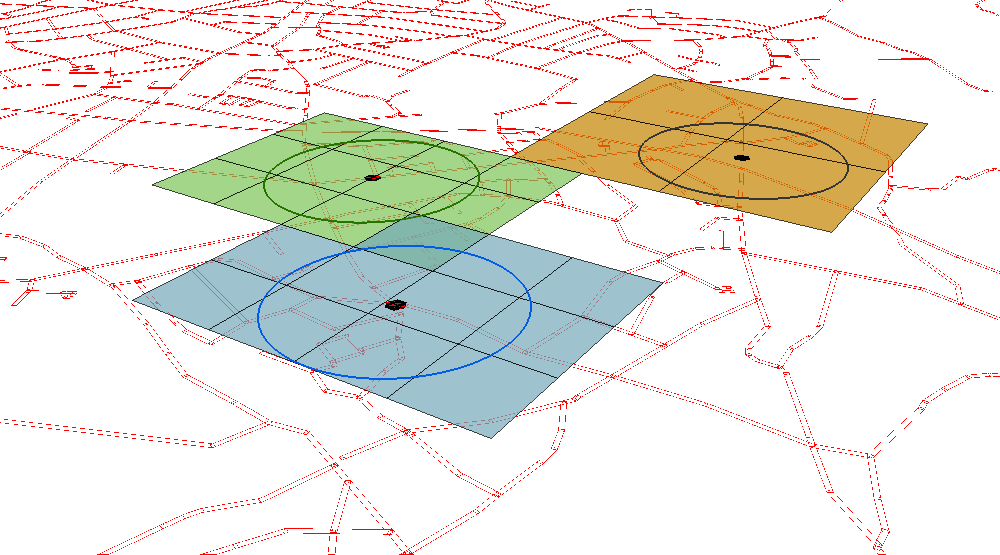
\includegraphics[page=1,scale=0.70]{images/demoVL/dump4.pdf}}
% 	\only<5>{ 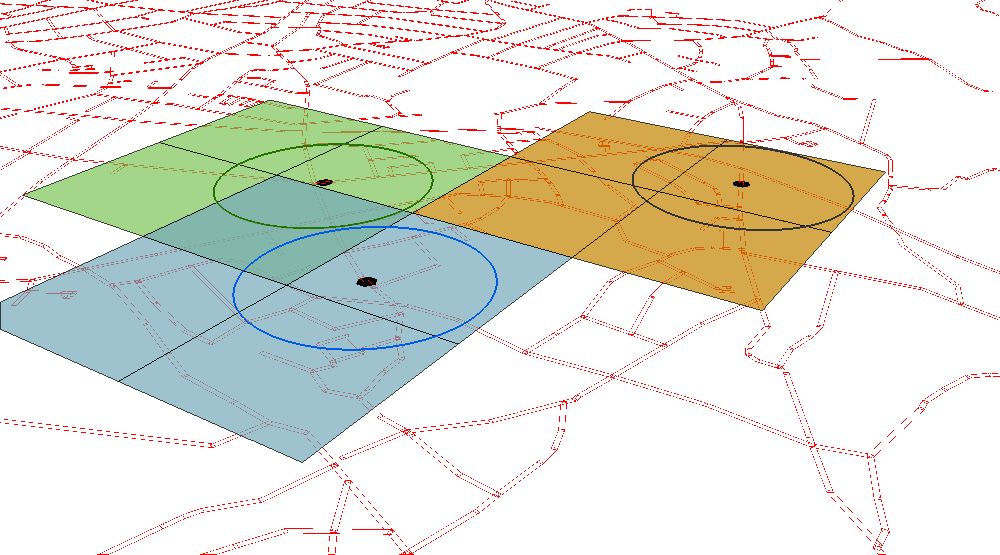
\includegraphics[page=1,scale=0.70]{images/demoVL/dump5.pdf}}
%   \only<6>{ 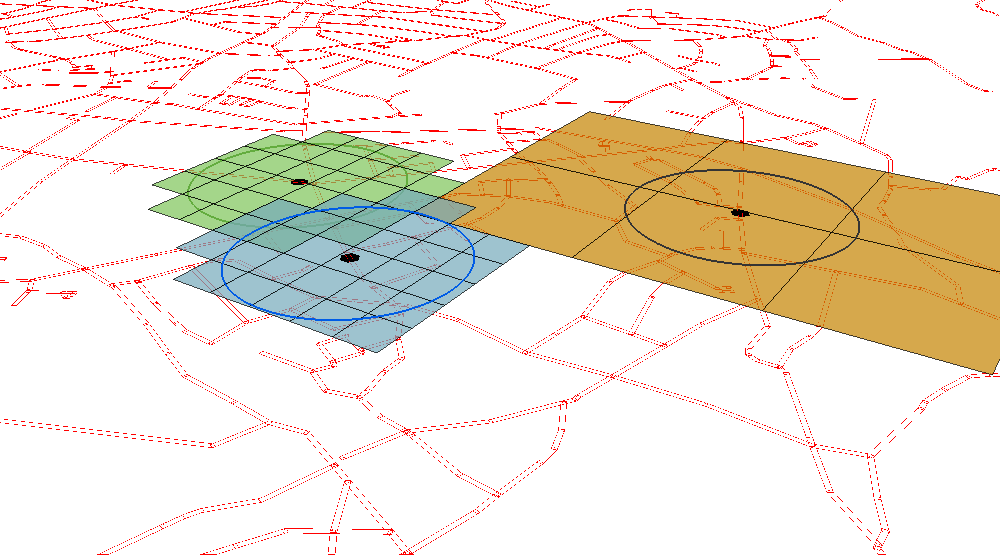
\includegraphics[page=1,scale=0.70]{images/demoVL/dump6.pdf}}	
%   \only<7>{ 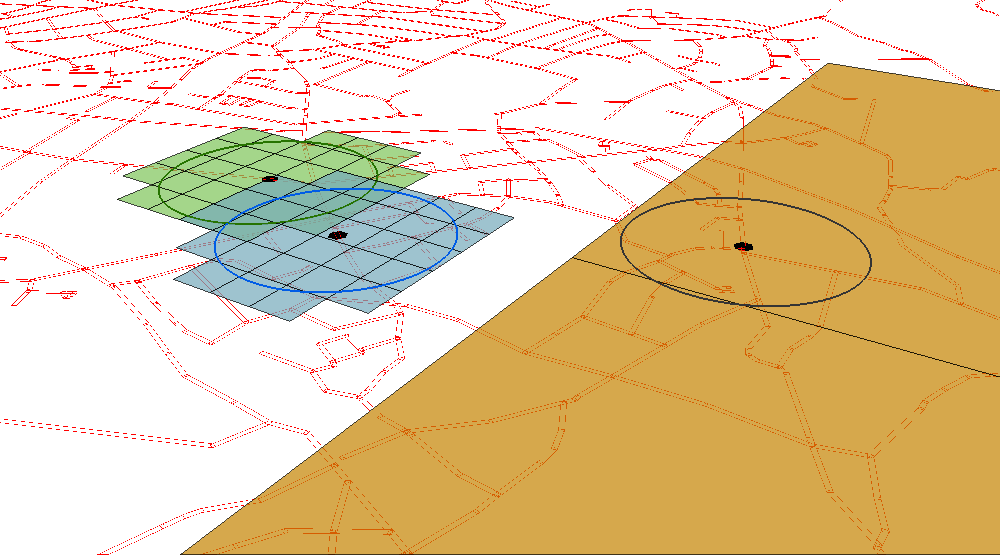
\includegraphics[page=1,scale=0.70]{images/demoVL/dump7.pdf}}	
%   \only<8>{ 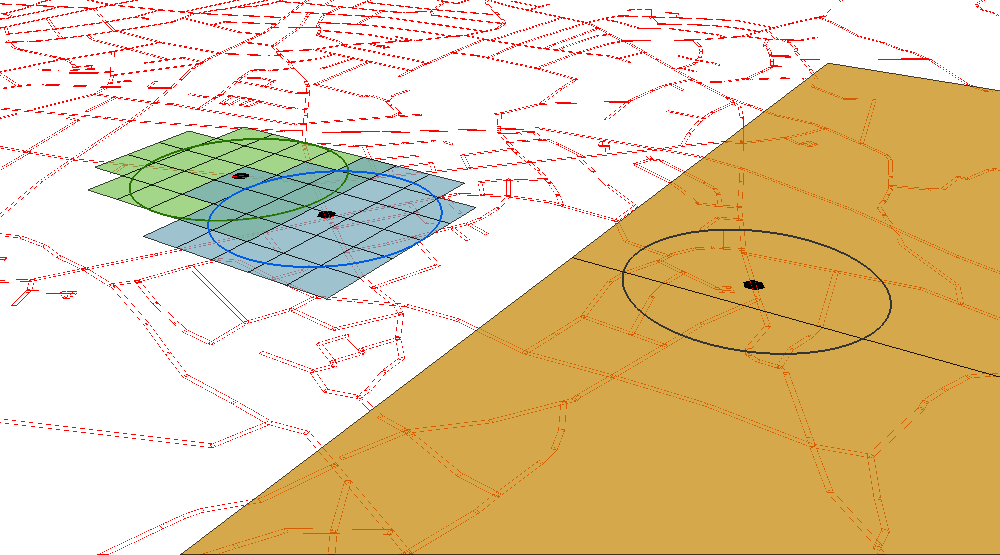
\includegraphics[page=1,scale=0.70]{images/demoVL/dump8.pdf}}	  
% \end{frame}
% 
% 
% \begin{frame}[red] %hmm.. thought i could change colour here :S
% \frametitle{\textsc{VicinityLocator} with Roadnetwork Filter}
% 
% \end{frame}
% 
% 
% \begin{frame}[red] %hmm.. thought i could change colour here :S
% \frametitle{Demo of \textsc{VicinityLocator} with Roadnetwork Filter}% R=800, Lmax = 8}
% 	\only<1>{ 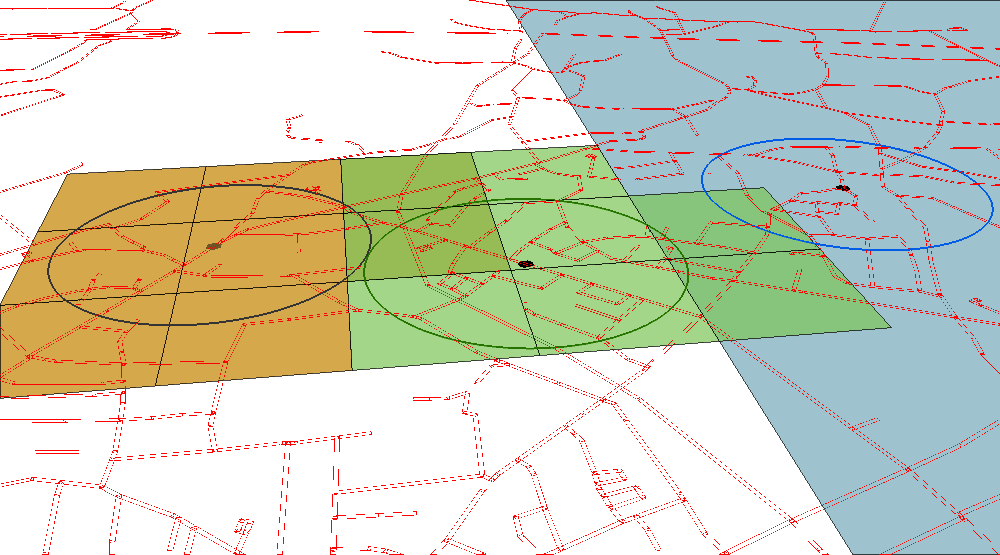
\includegraphics[page=1,scale=0.70]{images/demoVLRN/dump2.pdf}}
% 	\only<2>{ 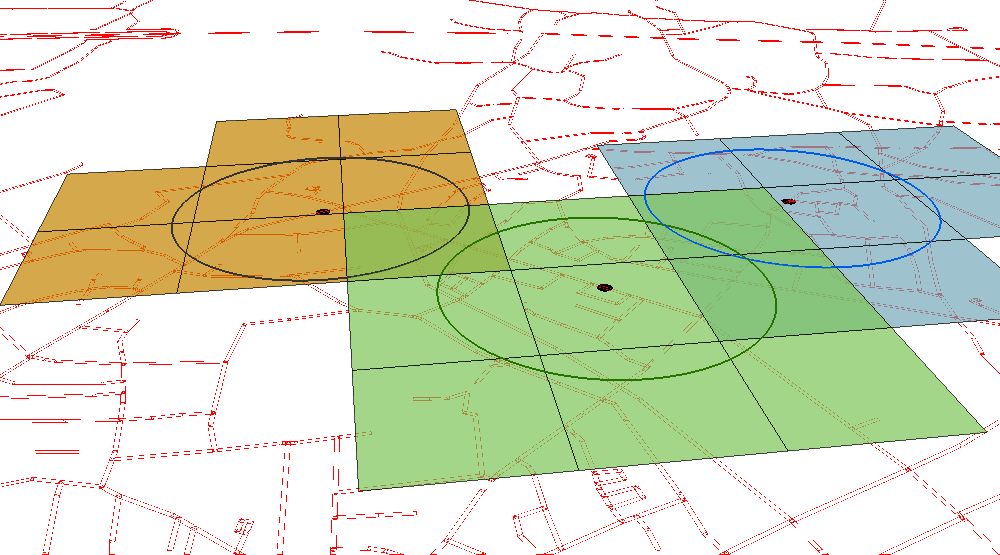
\includegraphics[page=1,scale=0.70]{images/demoVLRN/dump3.pdf}}
% 	\only<3>{ 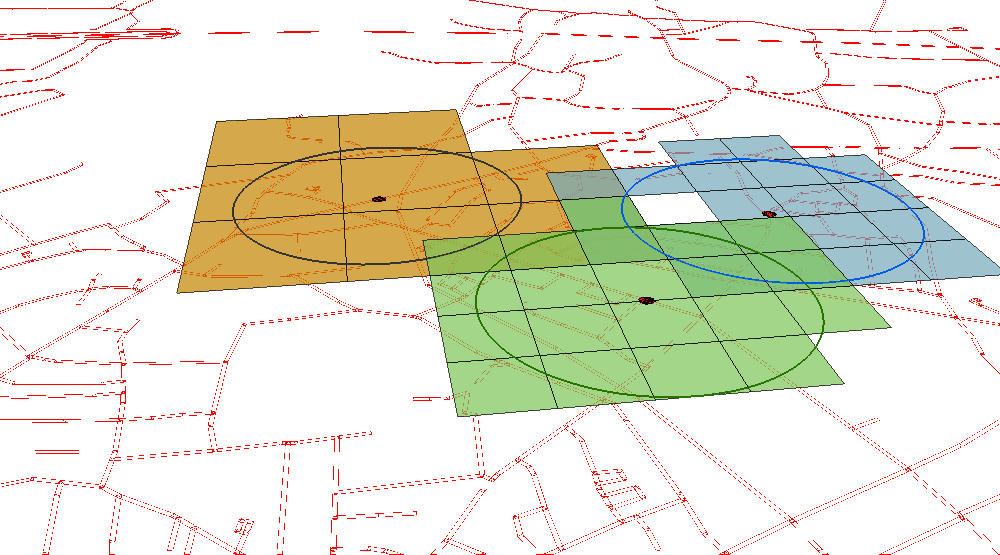
\includegraphics[page=1,scale=0.70]{images/demoVLRN/dump4.pdf}}
% 	\only<4>{ 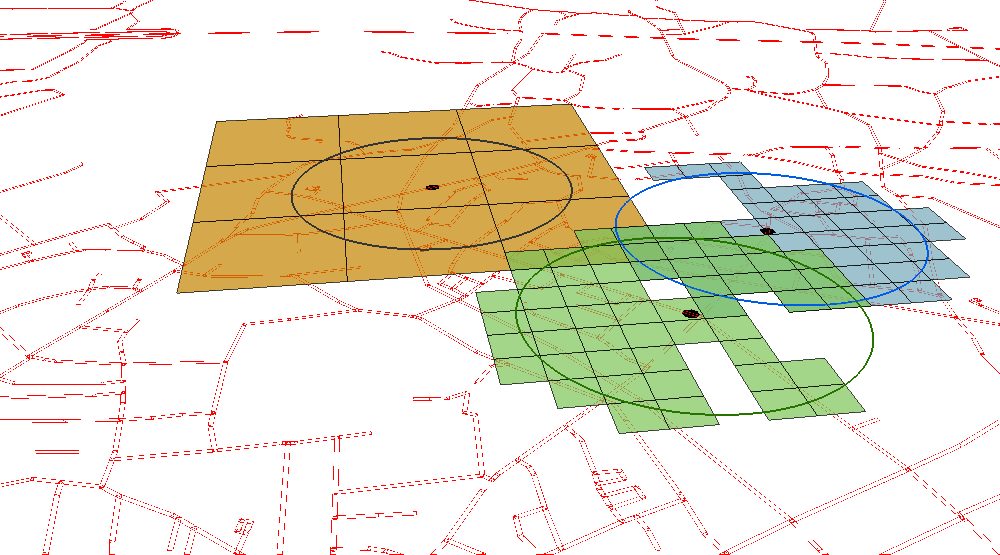
\includegraphics[page=1,scale=0.70]{images/demoVLRN/dump5.pdf}}
%   \only<5>{ 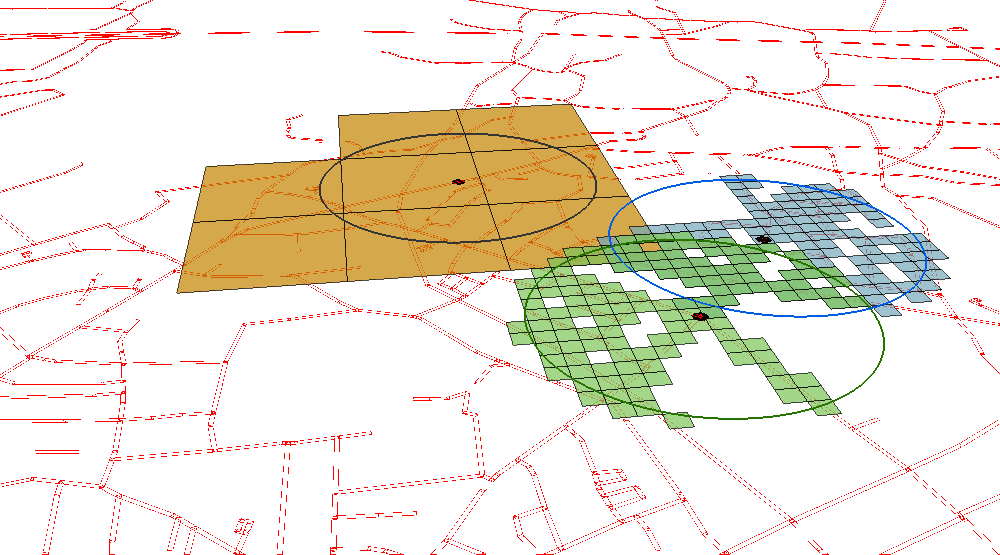
\includegraphics[page=1,scale=0.70]{images/demoVLRN/dump6.pdf}}	
%   \only<6>{ 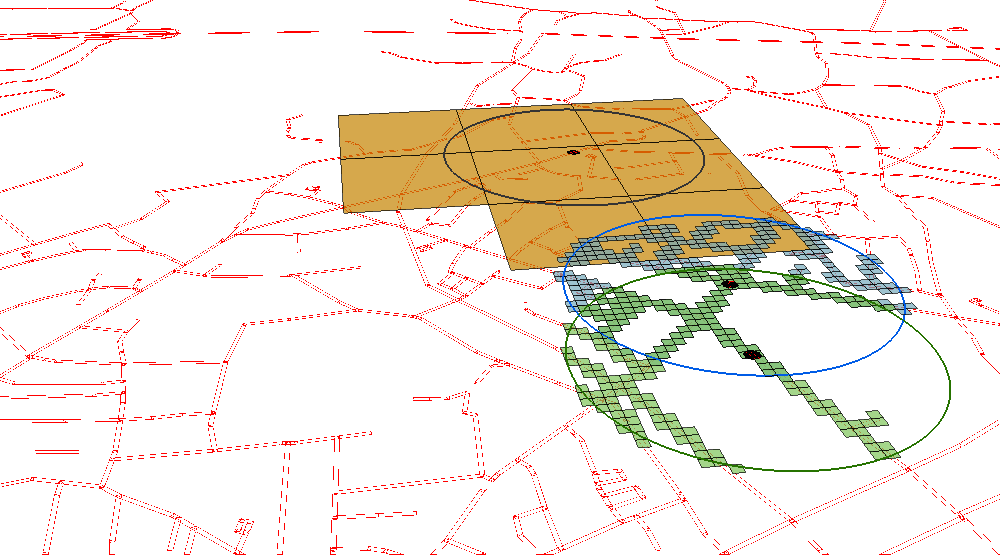
\includegraphics[page=1,scale=0.70]{images/demoVLRN/dump7.pdf}}		  
% \end{frame}
% 
% \begin{frame}[red] %hmm.. thought i could change colour here :S
% \frametitle{\textsc{VicinityLocator} with Incremental Update}
% 
% \begin{columns}
% \begin{column}{0.5\textwidth}
% \begin{itemize}
% \item Incremental Update
% \end{itemize}
% \vspace{5cm}
% \end{column}
% \begin{column}{0.5\textwidth}
% \pgfputat{\pgfxy(0,0)}{\pgfbox[left,top]{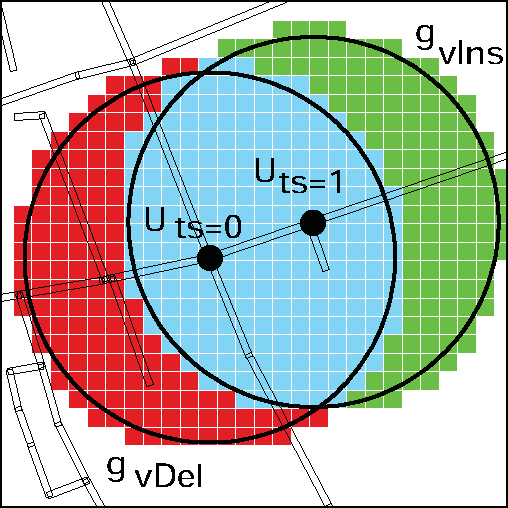
\includegraphics[width=1.1\textwidth]{images/incUpdDemo.pdf}}}
% \end{column}
% \end{columns}
% \end{frame}
% 
% 
% \begin{frame}[red] %hmm.. thought i could change colour here :S
% \frametitle{\textsc{VicinityLocator} with Incremental Update}
% 
% \begin{columns}
% \begin{column}{0.5\textwidth}
% \begin{itemize}
% \item Incremental Update \& Roadnetwork Filter
% \end{itemize}
% \vspace{5cm}
% \end{column}
% \begin{column}{0.5\textwidth}
% \pgfputat{\pgfxy(0,0)}{\pgfbox[left,top]{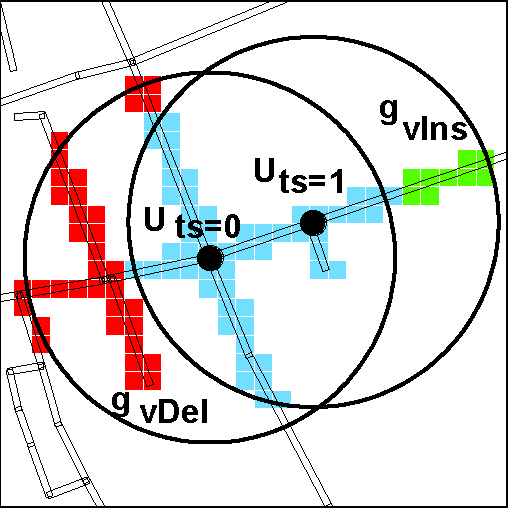
\includegraphics[width=1.1\textwidth]{images/incUpdDemo2.pdf}}}
% \end{column}
% \end{columns}
% \end{frame}
%\section{Experimental Results}

\begin{frame}
\frametitle{Setting} %Intro/purpose of this section}

\begin{itemize}
\item .
\end{itemize}

\end{frame}

\subsection{$B^+$-Tree}

\begin{frame}
\frametitle{SS}

\begin{itemize}
\item .
\end{itemize}

\end{frame}
\subsection{Hash Join}

\begin{frame}
\frametitle{SS}

\begin{itemize}
\item .
\end{itemize}

\end{frame}



\subsection{Conclusion}

\begin{frame}
\frametitle{SS}

\begin{itemize}
\item .
\end{itemize}

\end{frame}
\section{Conclusion and Future Work}\label{sec:future}



summation of each goal from the problem setting for each goal argue we solved it well (recap key results and partial conclusions from applicable sections).






% In this paper we develop a novel Privacy Profile which enable users to easily specify their privacy requirements both spatially and temporally for trajectories.
% 
% To show the Privacy Profile usefull we develop framework with a high level of user privacy and providing a platform for service providers and traffic analysts to have high quality data to perform analysis and services on.
% 
% We have argued that the Privacy Profile provide: 
% {\it Usability} The user can specify his privacy requirements both spatially and temporally, and at more than one level. Is {\it Practical} The user does not need to interact with the client once a Privacy Profile is set up. The data input format is the same as the data output format making the anonymized data usable by existing approaches working on trajectory datasets allowing the user to choose from more existing services. It is {\it Flexible} Users can specify sensitivity at several levels and they can make several profiles which are active at different times or in contexts.
% 
% We have additionally introduced the system parameter $\mathbf{D}$ which guaranties a minimum level of data integrity, ensuring that analysis of the anonymized dataset can still be possible.
% 
% In the future it would be interresting to test the approach on real world trajectory dataset to measure performance and examine which values of $D$ might be appropriate to ensure a level of data quality usable by existing classification approaches for trajectories.

\end{document}
